%!TEX root=./LIVRO.tex
\setcounter{chapter}{0}
\chapter[Simulado 1]{Simulado}
\markboth{Simulado 1}{}

\num{1} OBSERVE OS AGRUPAMENTOS A SEGUIR.

\begin{figure}[H]
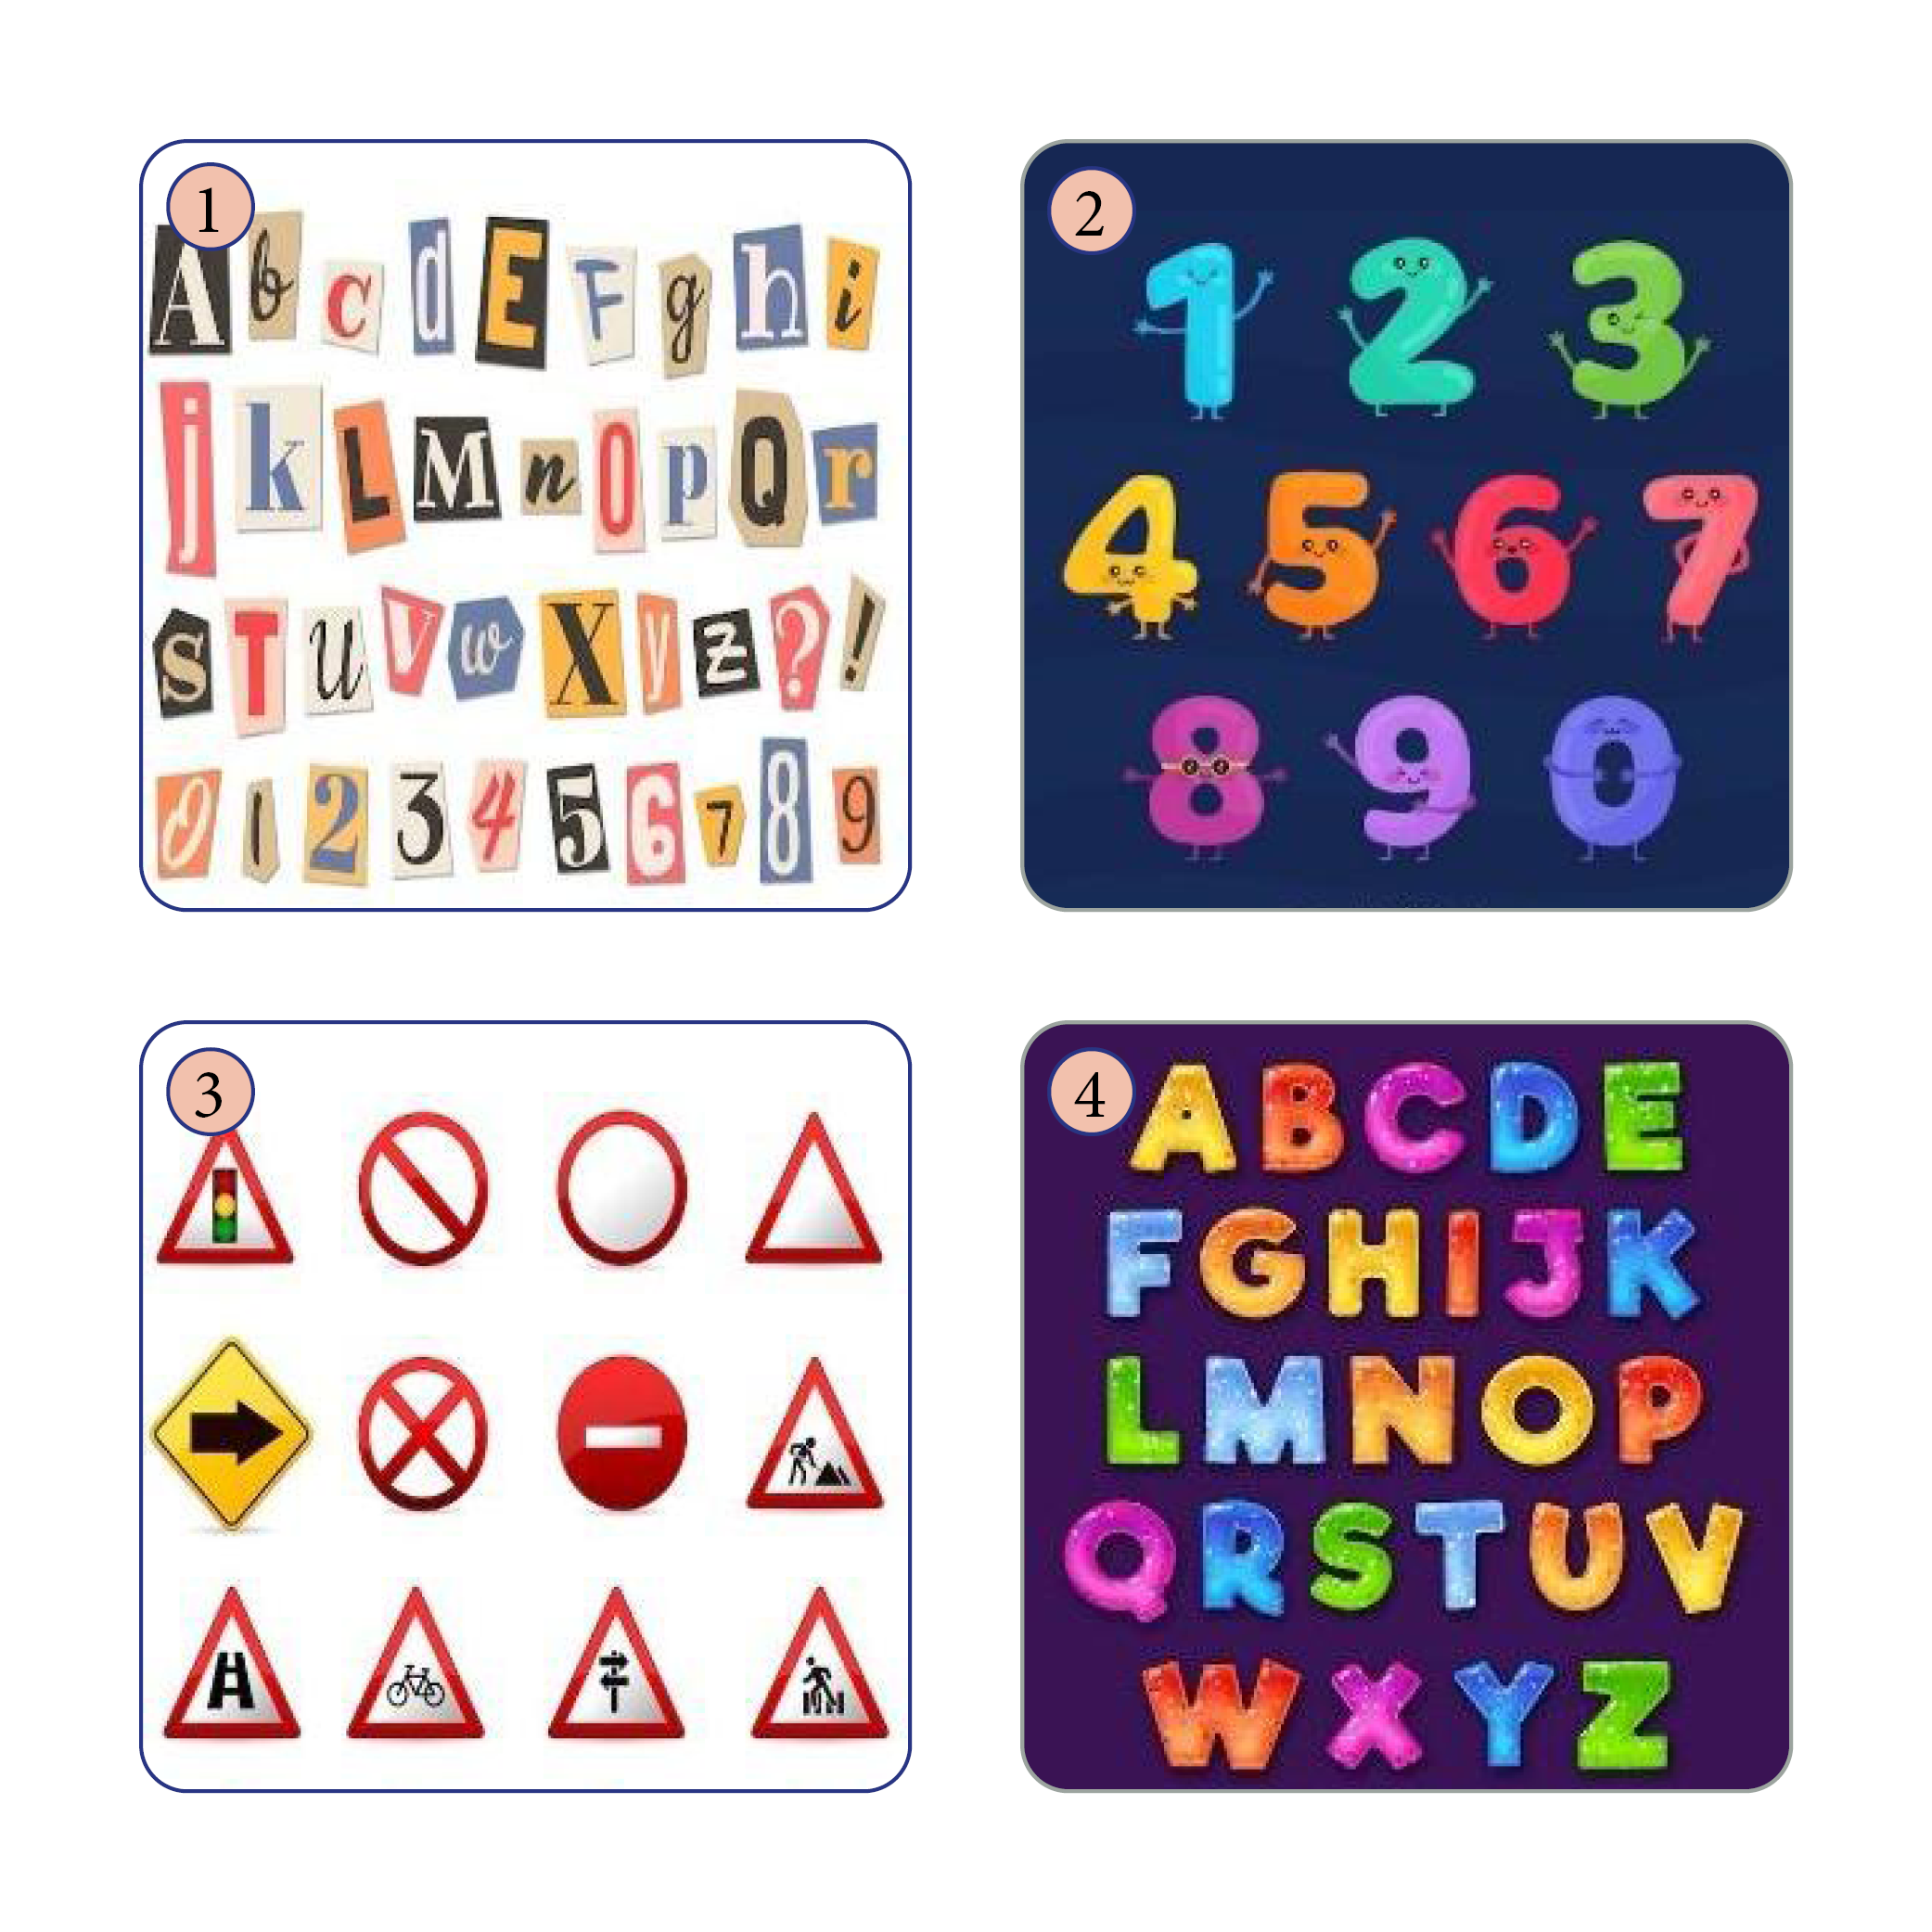
\includegraphics[width=\textwidth]{media/image183a186}
\end{figure}

O AGRUPAMENTO EM QUE SÓ APARECEM LETRAS É O

%\begin{multicols}{2}
\begin{escolha}
\item SUPERIOR ESQUERDO.

\item SUPERIOR DIREITO.

\item INFERIOR ESQUERDO.

\item INFERIOR DIREITO.
\end{escolha}
%\end{multicols}

\pagebreak

\num{2} QUAL DAS PALAVRAS A SEGUIR TEM A MESMA QUANTIDADE DE SONS QUE A PALAVRA \textbf{BOLA}?

%\begin{multicols}{2}
\begin{escolha}[itemsep=-5pt]
\item MACACO.

\item BONECA.

\item PATINETE.

\item PIPA.
\end{escolha}
%\end{multicols}

\num{3} VEJA A REPRESENTAÇÃO DO ANIMAL DE ESTIMAÇÃO QUE DANIEL GANHOU.

\begin{minipage}{.4\textwidth}
\begin{figure}[H]
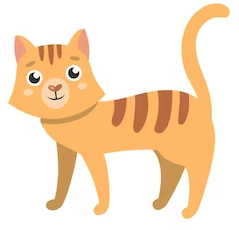
\includegraphics[width=\textwidth]{media/image187.png}
\end{figure}
\end{minipage}
\begin{minipage}{.5\textwidth}
O NOME DO ANIMAL COMEÇA COM 

\begin{escolha}
\item R.

\item P.

\item G .

\item K.
\end{escolha}
\end{minipage}

\vspace{0.5cm}

\num{4} VEJA OS CHINELOS QUE LÚCIA GANHOU DA AVÓ. 

\begin{minipage}{.3\textwidth}
\begin{figure}[H]
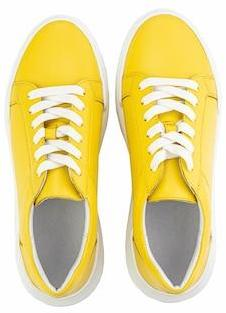
\includegraphics[width=\textwidth]{media/image189.jpg}
\end{figure}
\end{minipage}
\hspace{1cm}
\begin{minipage}{.7\textwidth}
QUAL É A SÍLABA FINAL DO NOME DA COR DO PAR DE CHINELOS QUE LÚCIA GANHOU?

\begin{escolha}
\item MA.

\item RE.

\item LO.

\item LU.
\end{escolha}
\end{minipage}

\pagebreak

\num{5} VEJA A PALAVRA QUE JÚLIA LEU PARA SUA PRIMA.

\begin{myquote}
\centering\LARGE{SALAME}
\end{myquote}

A PALAVRA A SEGUIR QUE NÃO TEM UMA SÍLABA COMO A MEDIAL
DA PALAVRA QUE JÚLIA LEU É

%\begin{multicols}{2}
\begin{escolha}%[itemsep=0pt]
\item SALADA.

\item SACOLA.

\item LÂMPADA.

\item PANELA.
\end{escolha}
%\end{multicols}

\num{6} VEJA O PRESENTE QUE TOMAS GANHOU DO SEU AMIGO.

\begin{figure}[H]
\centering
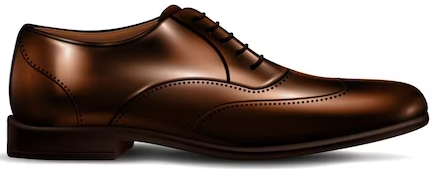
\includegraphics[width=.7\textwidth]{media/image191.png}
\end{figure}

O NOME DO PRESENTE QUE TOMAS GANHOU É

%\begin{multicols}{2}
\begin{escolha}%[itemsep=0pt]
\item SALADA.

\item SAPATO.

\item TOMATE.

\item PANELA.
\end{escolha}
%\end{multicols}

\vspace{0.3cm}

\num{7} OBSERVE A FRUTA PREFERIDA DE SOFIA.

\begin{minipage}{.2\textwidth}
\begin{figure}[H]

\includegraphics[width=\textwidth]{media/image192.png}
\end{figure}
\end{minipage}
\hspace{1cm}
\begin{minipage}{.8\textwidth}
ASSINALE O NOME CORRETO DESSA FRUTA.

\begin{escolha}
\item ABACAXI.

\item ABXICA.

\item ACAXI.

\item ABACAI.
\end{escolha}
\end{minipage}

\vspace{0.5cm}

\num{8} VEJA A PALAVRA QUE GUTO ESCREVEU.

\begin{myquote}
\centering\LARGE{TAPETE}
\end{myquote}

INDIQUE A PALAVRA QUE TERMINA COM O MESMO SOM.

%\begin{multicols}{2}
\begin{escolha}%[itemsep=0pt]
\item GILETE.

\item PETECA.

\item TESOURA.

\item TAMANCO.
\end{escolha}
%\end{multicols}

\conteudo{PARA A QUESTÃO DE NÚMERO 8, É PRECISO CONSIDERAR QUE A PALAVRA ``SOM'' EQUIVALE A ``SÍLABA''. PORTANTO É ESPERADO ENCONTRAR UMA PALAVRA QUE TEM A MESMA SÍLABA FINAL QUE A PALAVRA ESCRITA POR GUTO.}

\pagebreak

\num{9} LEIA ESTA FRASE.

\begin{myquote}
\large\centering{O MENINO CHUTA A BOLA.}
\end{myquote}

A IMAGEM QUE REPRESENTA O QUE ESTÁ ESCRITO NA FRASE É

\begin{multicols}{2}
\begin{escolha}
\item 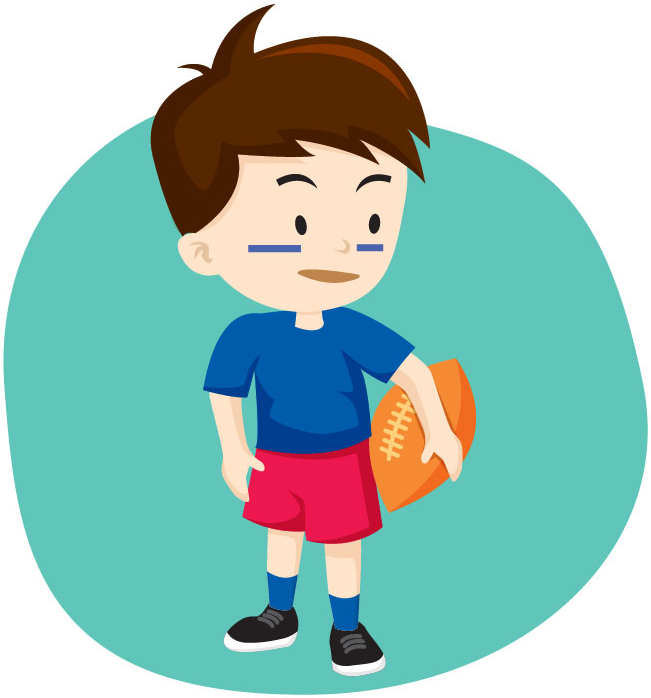
\includegraphics[width=.5\textwidth]{media/image258a.png}

\item 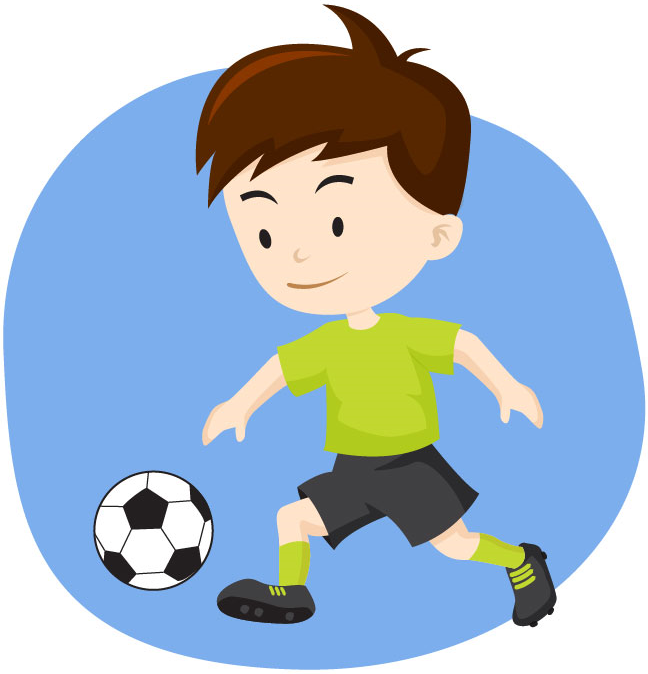
\includegraphics[width=.5\textwidth]{media/image258b.png}

\columnbreak

\item 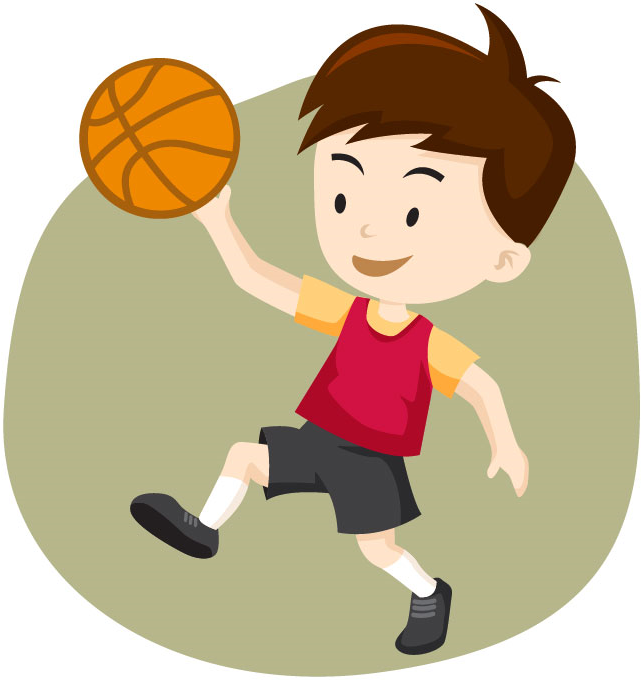
\includegraphics[width=.5\textwidth]{media/image258c.png}

\item 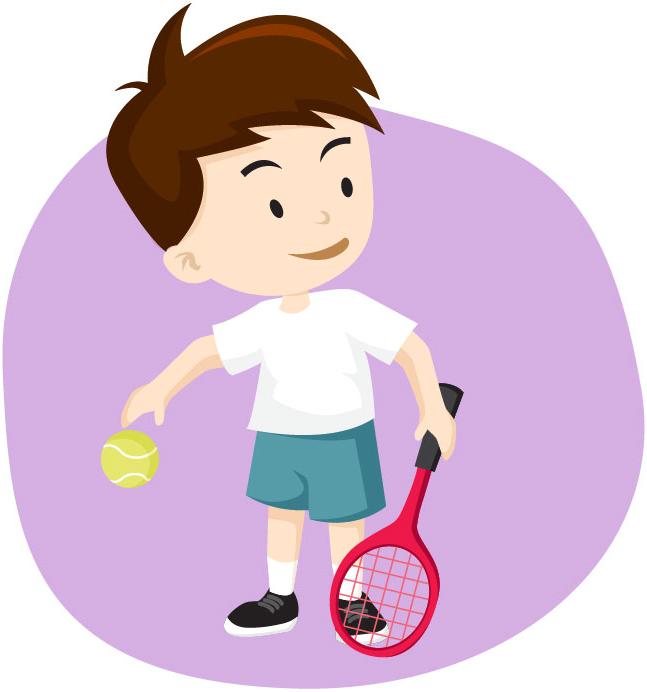
\includegraphics[width=.5\textwidth]{media/image258d.png}
\end{escolha}
\end{multicols}

\pagebreak

\num{10} LEIA O TEXTO.

\begin{myquote}
\begin{verse}
\textbf{O MEU CHAPÉU}

O MEU CHAPÉU TEM TRÊS PONTAS.\\
TEM TRÊS PONTAS O MEU CHAPÉU.\\
SE NÃO TIVESSE TRÊS PONTAS,\\
NÃO SERIA O MEU CHAPÉU.
\end{verse}

\fonte{DOMÍNIO PÚBLICO.}
\end{myquote}

O ASSUNTO DESSE TEXTO É

\begin{escolha}[itemsep=-5pt]
\item DESCOBRIR A QUEM PERTENCE O CHAPÉU.

\item MOSTRAR QUE O CHAPÉU NÃO SERVE PARA COLOCAR SOBRE A CABEÇA.

\item MOSTRAR QUE O CHAPÉU TEM MAIS QUE TRÊS PONTAS.

\item DESCREVER AS CARACTERÍSTICAS DO CHAPÉU.
\end{escolha}


\num{11} LEIA O TEXTO.

\begin{myquote}
\begin{verse}
\textbf{CORES E SABORES SEMANAIS}

NA TERÇA O PIMENTÃO SE MOSTRA NO AR,\\
NA QUARTA, O PÃO RECENTE A BRILHAR,\\
SABORES QUE DA FEIRA VÃO PARA O LAR.


NA QUINTA, NOVAS CORES A SE FORMAR,\\
SEXTA TRAZ FESTA AO PALADAR A VIBRAR,\\
SÁBADO PLENO, AROMAS A PERFUMAR,\\
DOMINGO, SATISFAÇÃO A NOS ABRAÇAR.
\end{verse}

\fonte{TEXTO ESCRITO PARA ESTE MATERIAL.}
\end{myquote}

%Disponível em:\textbf{\emph{\href{http://tinyurl.com/2b7fs26z. Acesso em: 18 fev. 2023. }}

\pagebreak

QUANDO SE PODEM COMPRAR PIMENTÃO E PÃO?

%\begin{multicols}{2}
\begin{escolha}
\item SÁBADO E DOMINGO.

\item DOMINGO E TERÇA.

\item QUARTA E SÁBADO.

\item TERÇA E QUARTA.
\end{escolha}
%\end{multicols}

\num{12} LARA VAI CONVIDAR ALICE PARA SEU ANIVERSÁRIO. 
QUAL TEXTO ELA DEVE MANDAR PARA SUA AMIGA? 

%\begin{multicols}{2}
\begin{escolha}
\item BILHETE.

\item CONVITE.

\item NOTÍCIA.

\item RECEITA.
\end{escolha}
%\end{multicols}

\begin{figure}[H]
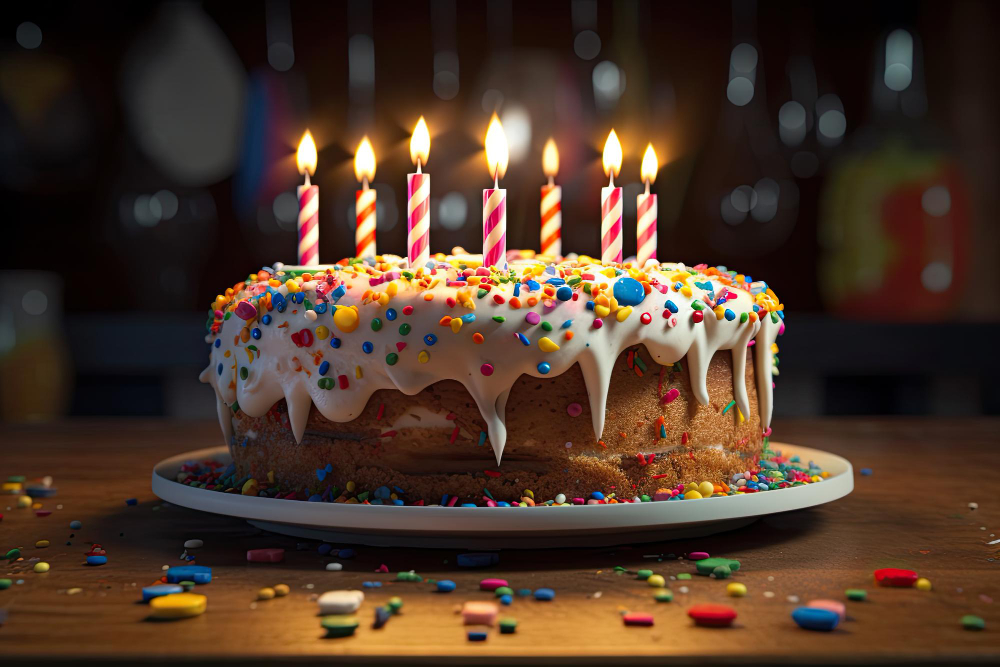
\includegraphics[width=\textwidth]{media/image269.png}
\end{figure}

\num{13} VEJA O CARTAZ.

\begin{figure}[H]
\centering
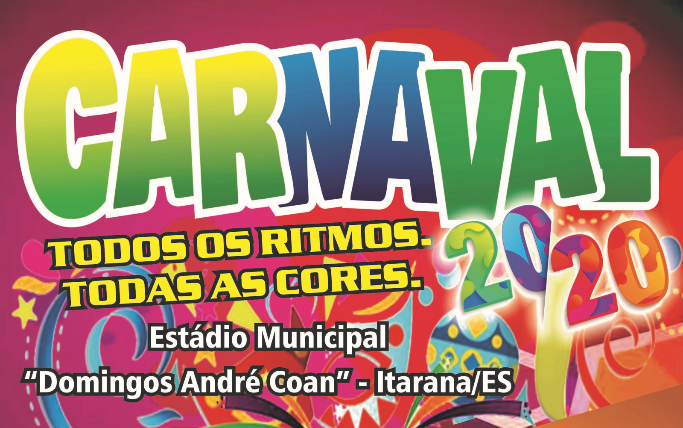
\includegraphics[width=.9\textwidth]{media/image204.png}
\end{figure}
%Disponível em:\href{https://www.itarana.es.gov.br/portal/artigo/prefeitura-municipal-de-itarana-apresenta-programacao-do-carnaval-2020-com-blocos-de-rua-e-shows-noturnos}{\emph{https://www.itarana.es.gov.br/portal/artigo/prefeitura-municipal-de-itarana-apresenta-programacao-do-carnaval-2020-com-blocos-de-rua-e-shows-noturnos}} Acesso em: 19 fev. 2023. 

ESSE TEXTO SERVE PARA

\begin{escolha}[itemsep=-5pt]
\item ORGANIZAR TAREFAS.

\item ENSINAR UMA RECEITA.

\item ANUNCIAR UM EVENTO.

\item CONTAR UMA HISTÓRIA.
\end{escolha}

\begin{figure}[H]
\centering
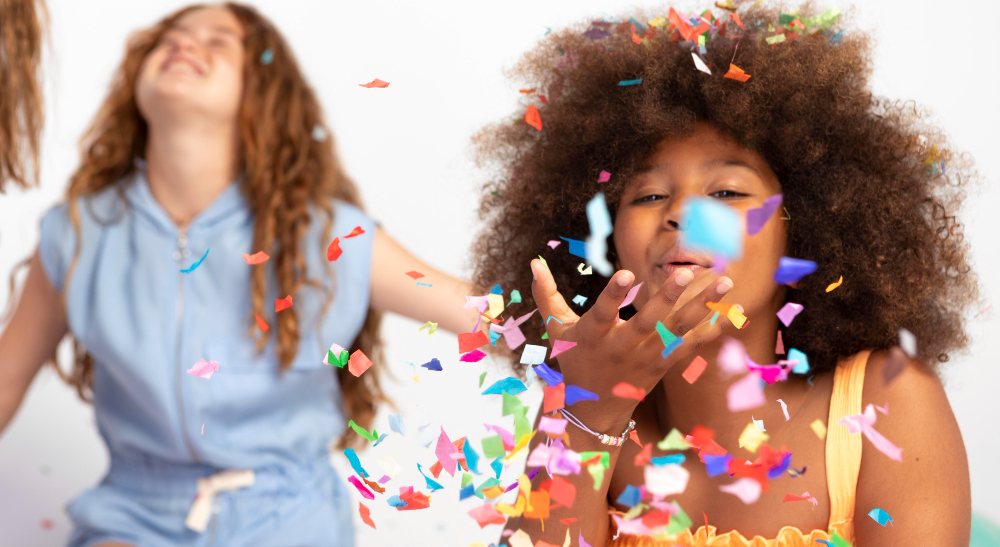
\includegraphics[width=.9\textwidth]{media/image270.png}
\end{figure}

\num{14} LEIA O TRECHO DA HISTÓRIA DE JOÃO E MARIA.

\begin{myquote}
NA MADRUGADA DO DIA SEGUINTE, A MADRASTA ACORDOU AS CRIANÇAS E FORAM
NOVAMENTE PARA A MATA. ENQUANTO CAMINHAVAM, JOÃOZINHO ESFARELOU TODO O
SEU PÃO E O DA IRMÃ, FAZENDO UMA TRILHA.

JOÃO E MARIA
ADORMECERAM, POR FOME E CANSAÇO E, QUANDO ACORDARAM, ESTAVA MUITO
ESCURO. MARIA DESATOU A CHORAR. E NÃO CONSEGUIRAM
ENCONTRAR O CAMINHO: OS PÁSSAROS DA MATA TINHAM COMIDO TODAS AS
MIGALHAS.

\fonte{DISPONÍVEL EM: \emph{http://www.dominiopublico.gov.br/download/texto/me001614.pdf}. ACESSO EM: 19 FEV. 2023.}
\end{myquote}

JOÃO FEZ A TRILHA DE PÃO PARA

\begin{escolha}[itemsep=-5pt]
\item ALIMENTAR OS PASSARINHOS.

\item CONSEGUIR VOLTAR PARA CASA.

\item COMER QUANDO SENTISSE FOME.

\item FUGIR DO PAI E DA MADASTRA.
\end{escolha}

\num{15} ANALISE O TEXTO.

% \begin{minipage}{.3\textwidth}
% 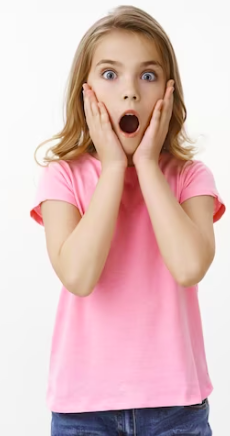
\includegraphics[width=\textwidth]{media/image205.png}
% \end{minipage}
% \begin{minipage}{.7\textwidth}
\begin{myquote}
--- NOSSA... ACABOU A LUZ! TENHO MEDO DO ESCURO!
\end{myquote}

COMO O PERSONAGEM FICOU QUANDO FALTOU LUZ?

%\begin{multicols}{2}
\begin{escolha}[itemsep=-5pt]
\item TRISTE.

\item ANIMADO.

\item ASSUSTADO.

\item NERVOSO.
\end{escolha}
%\end{multicols}

\chapter[Simulado 2]{Simulado}
\markboth{Simulado 2}{}

\pagebreak

\num{1} MARIANA QUER MOSTRAR PARA SUA AMIGA BIA QUE JÁ SABE ESCREVER O NOME DA SUA GATINHA MILU. PARA ISSO, ELA VAI ESCOLHER UMA MALETA DE SÍMBOLOS. 

\begin{figure}[H]
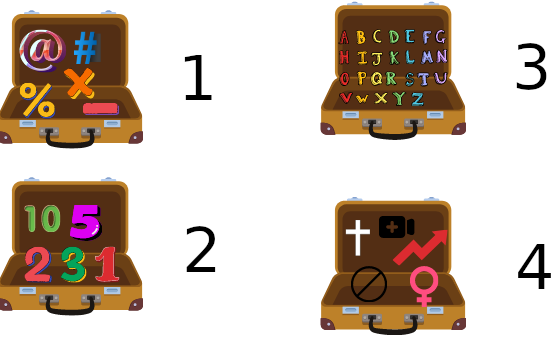
\includegraphics[width=\textwidth]{media/image209.png}
\end{figure}

MARIANA DEVE ESCOLHER A MALETA NÚMERO

\begin{multicols}{4}
\begin{escolha}[itemsep=0pt]
\item 1.

\item 2.

\item 3.

\item 4.
\end{escolha}
\end{multicols}

\num{2} OBSERVE O NOME DA FRUTA PREFERIDA DE ALICE.

\begin{minipage}{.5\textwidth}
\begin{figure}[H]
\centering
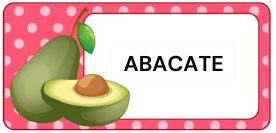
\includegraphics[width=\textwidth]{media/image212.png}
\end{figure}
\end{minipage}
\hspace{0.5cm}
\begin{minipage}{.5\textwidth}
QUAL PALAVRA APRESENTA AS MESMAS VOGAIS INICIAL E FINAL DO NOME DA FRUTA PREFERIDA DE ALICE?
\end{minipage}

\vspace{0.5cm}

\begin{multicols}{2}
\begin{escolha}[itemsep=0pt]
\item MACACO.

\item ÁRVORE.

\item COELHO.

\item GATO.
\end{escolha}
\end{multicols}

\pagebreak

\num{3} OBSERVE A PALAVRA QUE ANA APRENDEU A LER.

\begin{myquote}
\centering\large{FADA}
\end{myquote}

QUAL PALAVRA TEM A MESMA QUANTIDADE DE SONS?

\begin{multicols}{2}
\begin{escolha}[itemsep=0pt]
\item SALA.

\item TOMATE.

\item BONECA.

\item BICICLETA.
\end{escolha}
\end{multicols}

\num{4} VEJA A PALAVRA QUE MARINA LEU.

\begin{myquote}
\centering\large{BONECA}
\end{myquote}

AS LETRAS QUE FORMAM O SOM MEDIAL DA PALAVRA QUE ANA LEU SÃO

\begin{multicols}{4}
\begin{escolha}[itemsep=0pt]
\item B + O.

\item N + E.

\item C + A.

\item M + E.
\end{escolha}
\end{multicols}

\num{5} VEJA O ANIMAL DE ESTIMAÇÃO DE MIGUEL.

\begin{figure}[H]
\centering
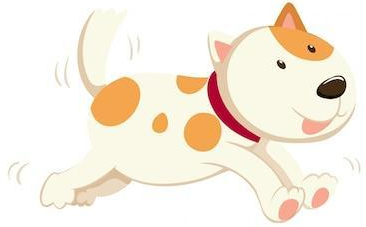
\includegraphics[width=.55\textwidth]{media/image214.jpg}
\end{figure}

A PALAVRA QUE COMEÇA COM A MESMA SÍLABA DO NOME DO ANIMAL É 

\begin{multicols}{2}
\begin{escolha}[itemsep=0pt]
\item CANECA.

\item BONECA.

\item CAVALO.

\item TUCANO.
\end{escolha}
\end{multicols}

\num{6} VEJA O ANIMAL QUE TIAGO ADOTOU PARA ALEGRAR SUA FAZENDA.

\begin{figure}[htpb]
\centering
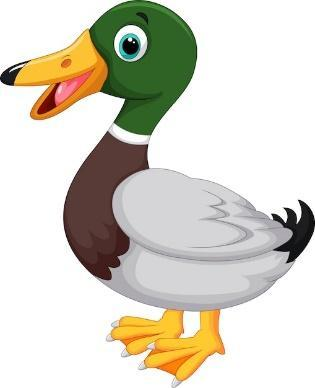
\includegraphics[width=.3\textwidth]{media/image215.jpg}
\end{figure}

A SÍLABA INICIAL DO NOME DESSE ANIMAL É

\begin{escolha}
\item GA.

\item TO.

\item BA.

\item PA.
\end{escolha}

\num{7} LEIA ESTA PALAVRA.

\begin{myquote}
\centering\large{PANELA}
\end{myquote}

A ÚLTIMA LETRA DESSA PALAVRA É

\begin{escolha}
\item P.

\item N.

\item E.

\item A.
\end{escolha}

%\pagebreak

\num{8} OBSERVE O QUE MONIQUE COMPROU PARA SUA COLEÇÃO.

\begin{figure}[H]
\centering
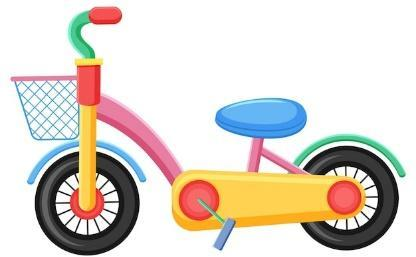
\includegraphics[width=.3\textwidth]{media/image217.jpg}
\end{figure}

O NOME DO BRINQUEDO QUE ELA COMPROU É

\begin{escolha}
\item BISCOITO.

\item BICICLETA.

\item TRICICLO.

\item CANETA.
\end{escolha}

\num{9} OBSERVE A CENA.

\begin{figure}[H]
\centering
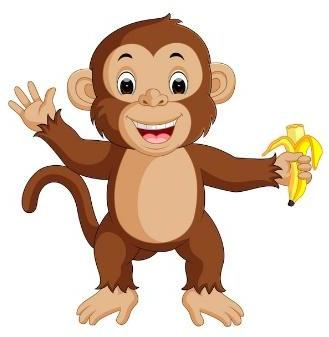
\includegraphics[width=.3\textwidth]{media/image218.jpg}
\end{figure}

QUAL FRASE REPRESENTA ESSA IMAGEM?

\begin{escolha}
\item O MACACO ESTÁ COMENDO A BANANA.

\item O MACACO JOGOU A BANANA NO CHÃO.

\item A BANANA DO MACACO CAIU.

\item A BANANA ESTÁ VERDE.
\end{escolha}

%\pagebreak
\num{10} VEJA O ANIMAL QUE PEDRO GOSTA DE VISITAR NO ZOOLÓGICO.

\begin{minipage}{.5\textwidth}
\begin{figure}[H]
\centering
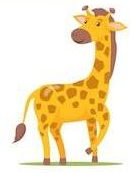
\includegraphics[width=.5\textwidth]{media/image219.jpg}
\end{figure}
\end{minipage}
\hspace{0.5cm}
\begin{minipage}{.5\textwidth}
O NOME DESSE ANIMAL É

\begin{escolha}
\item GIRAFA.

\item IRAFA.

\item GIRFA.

\item FIRAGA.
\end{escolha}
\end{minipage}

\vspace{0.5cm}

\num{11} LEIA O TEXTO.

\begin{myquote}
\begin{verse}
\textbf{A CASA FEIA}

O GATO FEZ UMA CASA\\
VEIO O RATO E FALOU:\\
--- HUM! QUE CASA FEIA!\\
CASA BONITA TEM TELHADO,\\
LOGO, LOGO O GATO FEZ O TELHADO.\\
VEIO O PATO E FALOU:\\
--- HUM QUE CASA FEIA!\\
CASA BONITA TEM VARANDA.\\
O GATO FEZ UMA VARANDA.\\
VEIO O BODE E FALOU:\\
--- HUM... QUE CASA FEIA!\\
CASA BONITA É PINTADA.\\
E O GATO PINTOU A CASA.\\
--- HUM... CASA BONITA TEM JARDIM.\\
\end{verse}

\fonte{DISPONÍVEL EM: \emph{https://tinyurl.com/y5mzt3x8}. ACESSO EM: 14 ABR. 2023.}
\end{myquote}	

QUEM DISSE AO GATO QUE CASA BONITA TEM VARANDA? 

\begin{multicols}{2}
\begin{escolha}
\item RATO.

\item GATO.

\item PATO.

\item BODE.
\end{escolha}
\end{multicols}

\begin{figure}[H]
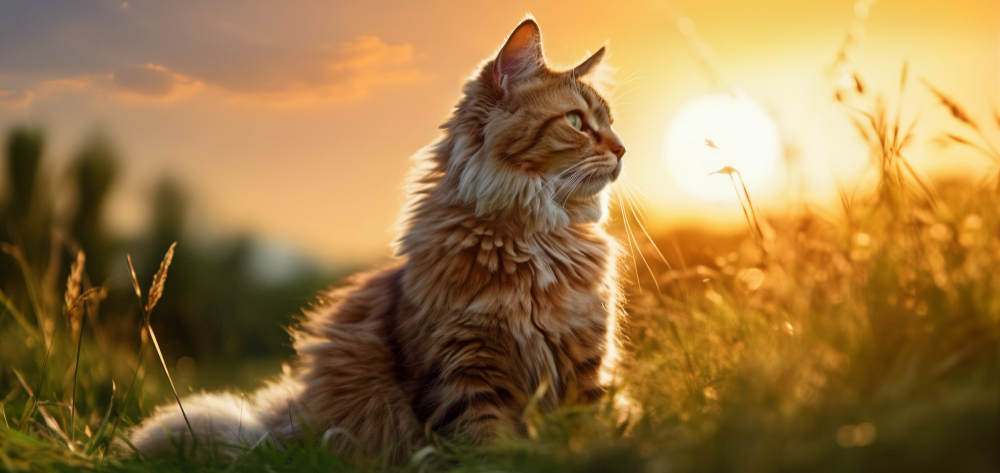
\includegraphics[width=\textwidth]{media/image271.png}
\end{figure}

\num{12} LEIA O TEXTO.

\begin{myquote}
\begin{verse}
\textbf{A BARATA}

A BARATA DIZ QUE TEM\\
SETE SAIAS DE FILÓ.\\
É MENTIRA DA BARATA.\\
ELA TEM É UMA SÓ.


A BARATA DIZ QUE TEM\\
SETE SAIAS DE BALÃO.\\
É MENTIRA! ELA NÃO TEM\\
NEM DINHEIRO PRO SABÃO.
\end{verse}

\fonte{DOMÍNIO PÚBLICO.}
\end{myquote}

\pagebreak

QUAL É O ASSUNTO DESSE TEXTO?

%\begin{multicols}{2}
\begin{escolha}
\item O DINHEIRO DA BARATA.

\item A MENTIRA DA BARATA.

\item O DESEJO DA BARATA.

\item A INVEJA DA BARATA.
\end{escolha}
%\end{multicols}

\num{13} OBSERVE O TEXTO.

\begin{figure}[htpb]
\centering
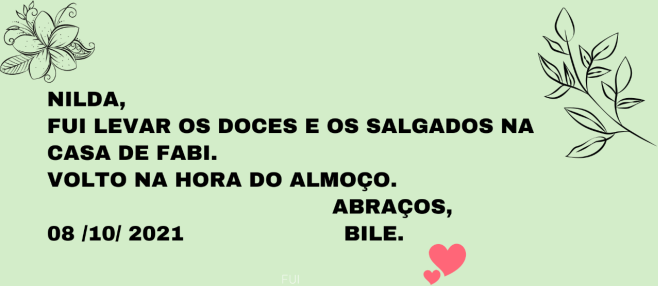
\includegraphics[width=\textwidth]{media/image220.png}
\end{figure}
%ELABORADO PELA AUTORA

ESSE TEXTO SERVE PARA

\begin{escolha}
\item DEIXAR UM RECADO.

\item DIVULGAR UM EVENTO.

\item ORGANIZAR AS TAREFAS.

\item ENSINAR A FAZER UMA COMIDA.
\end{escolha}

\pagebreak

\num{14} LEIA O TEXTO:

\begin{myquote}
\textbf{O LEÃO E O RATINHO}


UM LEÃO DORMIA À SOMBRA
DE UMA BOA ÁRVORE. VIERAM UNS RATINHOS PASSEAR EM CIMA DELE
E ELE ACORDOU. SÓ UM NÃO CONSEGUIU FUGIR, QUE O LEÃO
PRENDEU. TANTO O RATINHO IMPLOROU
QUE O LEÃO DESISTIU DE ESMAGÁ-LO E O DEIXOU IR.
ALGUM TEMPO DEPOIS, O LEÃO FICOU PRESO NUMA REDE. APARECEU O RATINHO,
QUE ROEU AS CORDAS E SOLTOU O LEÃO.

\fonte{DISPONÍVEL EM: \emph{http://www.dominiopublico.gov.br/download/texto/me001614.pdf}. ACESSO EM: 
20 FEV. 2023.}
\end{myquote}

O RATINHO AJUDOU O LEÃO PORQUE ELE

\begin{escolha}
\item ERA MUITO BONZINHO E GENTIL.

\item ERA MUITO VALENTE E RAIVOSO.

\item TINHA O ESMAGADO UM DIA.

\item TINHA O AJUDADO NO PASSADO.
\end{escolha}

\begin{figure}[H]
\centering
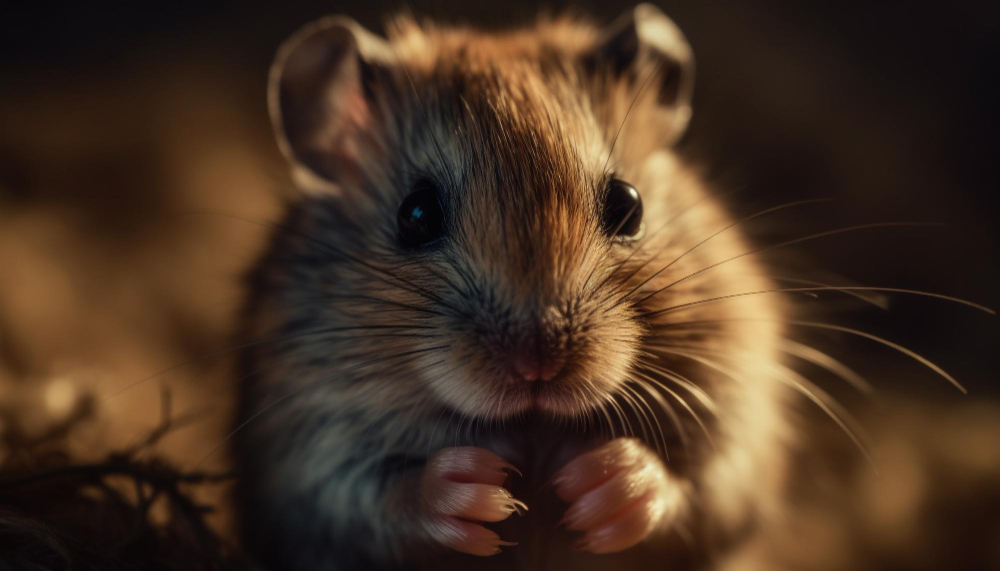
\includegraphics[width=.9\textwidth]{media/image272.png}
\end{figure}

\num{15} LEIA O DIÁLOGO E OBSERVE A IMAGEM.

\begin{figure}[H]
\centering
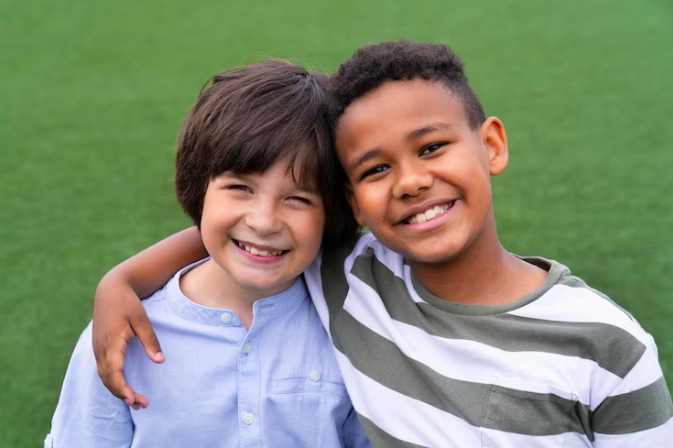
\includegraphics[width=\textwidth]{media/image220b.png}
\end{figure}

\begin{myquote}
BETO DISSE:

--- CHEGOU DE VIAGEM, LUCAS?

--- ISSO MESMO, BETO. CHEGUEI ONTEM À NOITE.

--- ENTÃO HOJE NÃO TEREI DE BRINCAR SOZINHO?

--- NÃO MESMO!

--- EBA!
\end{myquote}

BETO FICOU FELIZ PORQUE

\begin{escolha}
\item CHEGOU DE VIAGEM.

\item BRIGOU COM LUCAS.

\item BRINCOU ONTEM À NOITE.

\item TEM UM AMIGO PRA BRINCAR.
\end{escolha}



\chapter[Simulado 3]{Simulado}
\markboth{Simulado 3}{}

\pagebreak

\num{1} IZABEL VAI ESCOLHER UMA PLACA PARA ESCREVER O SEU NOME EM UM JOGO. QUAL ELA DEVE ESCOLHER?

\begin{figure}[H]
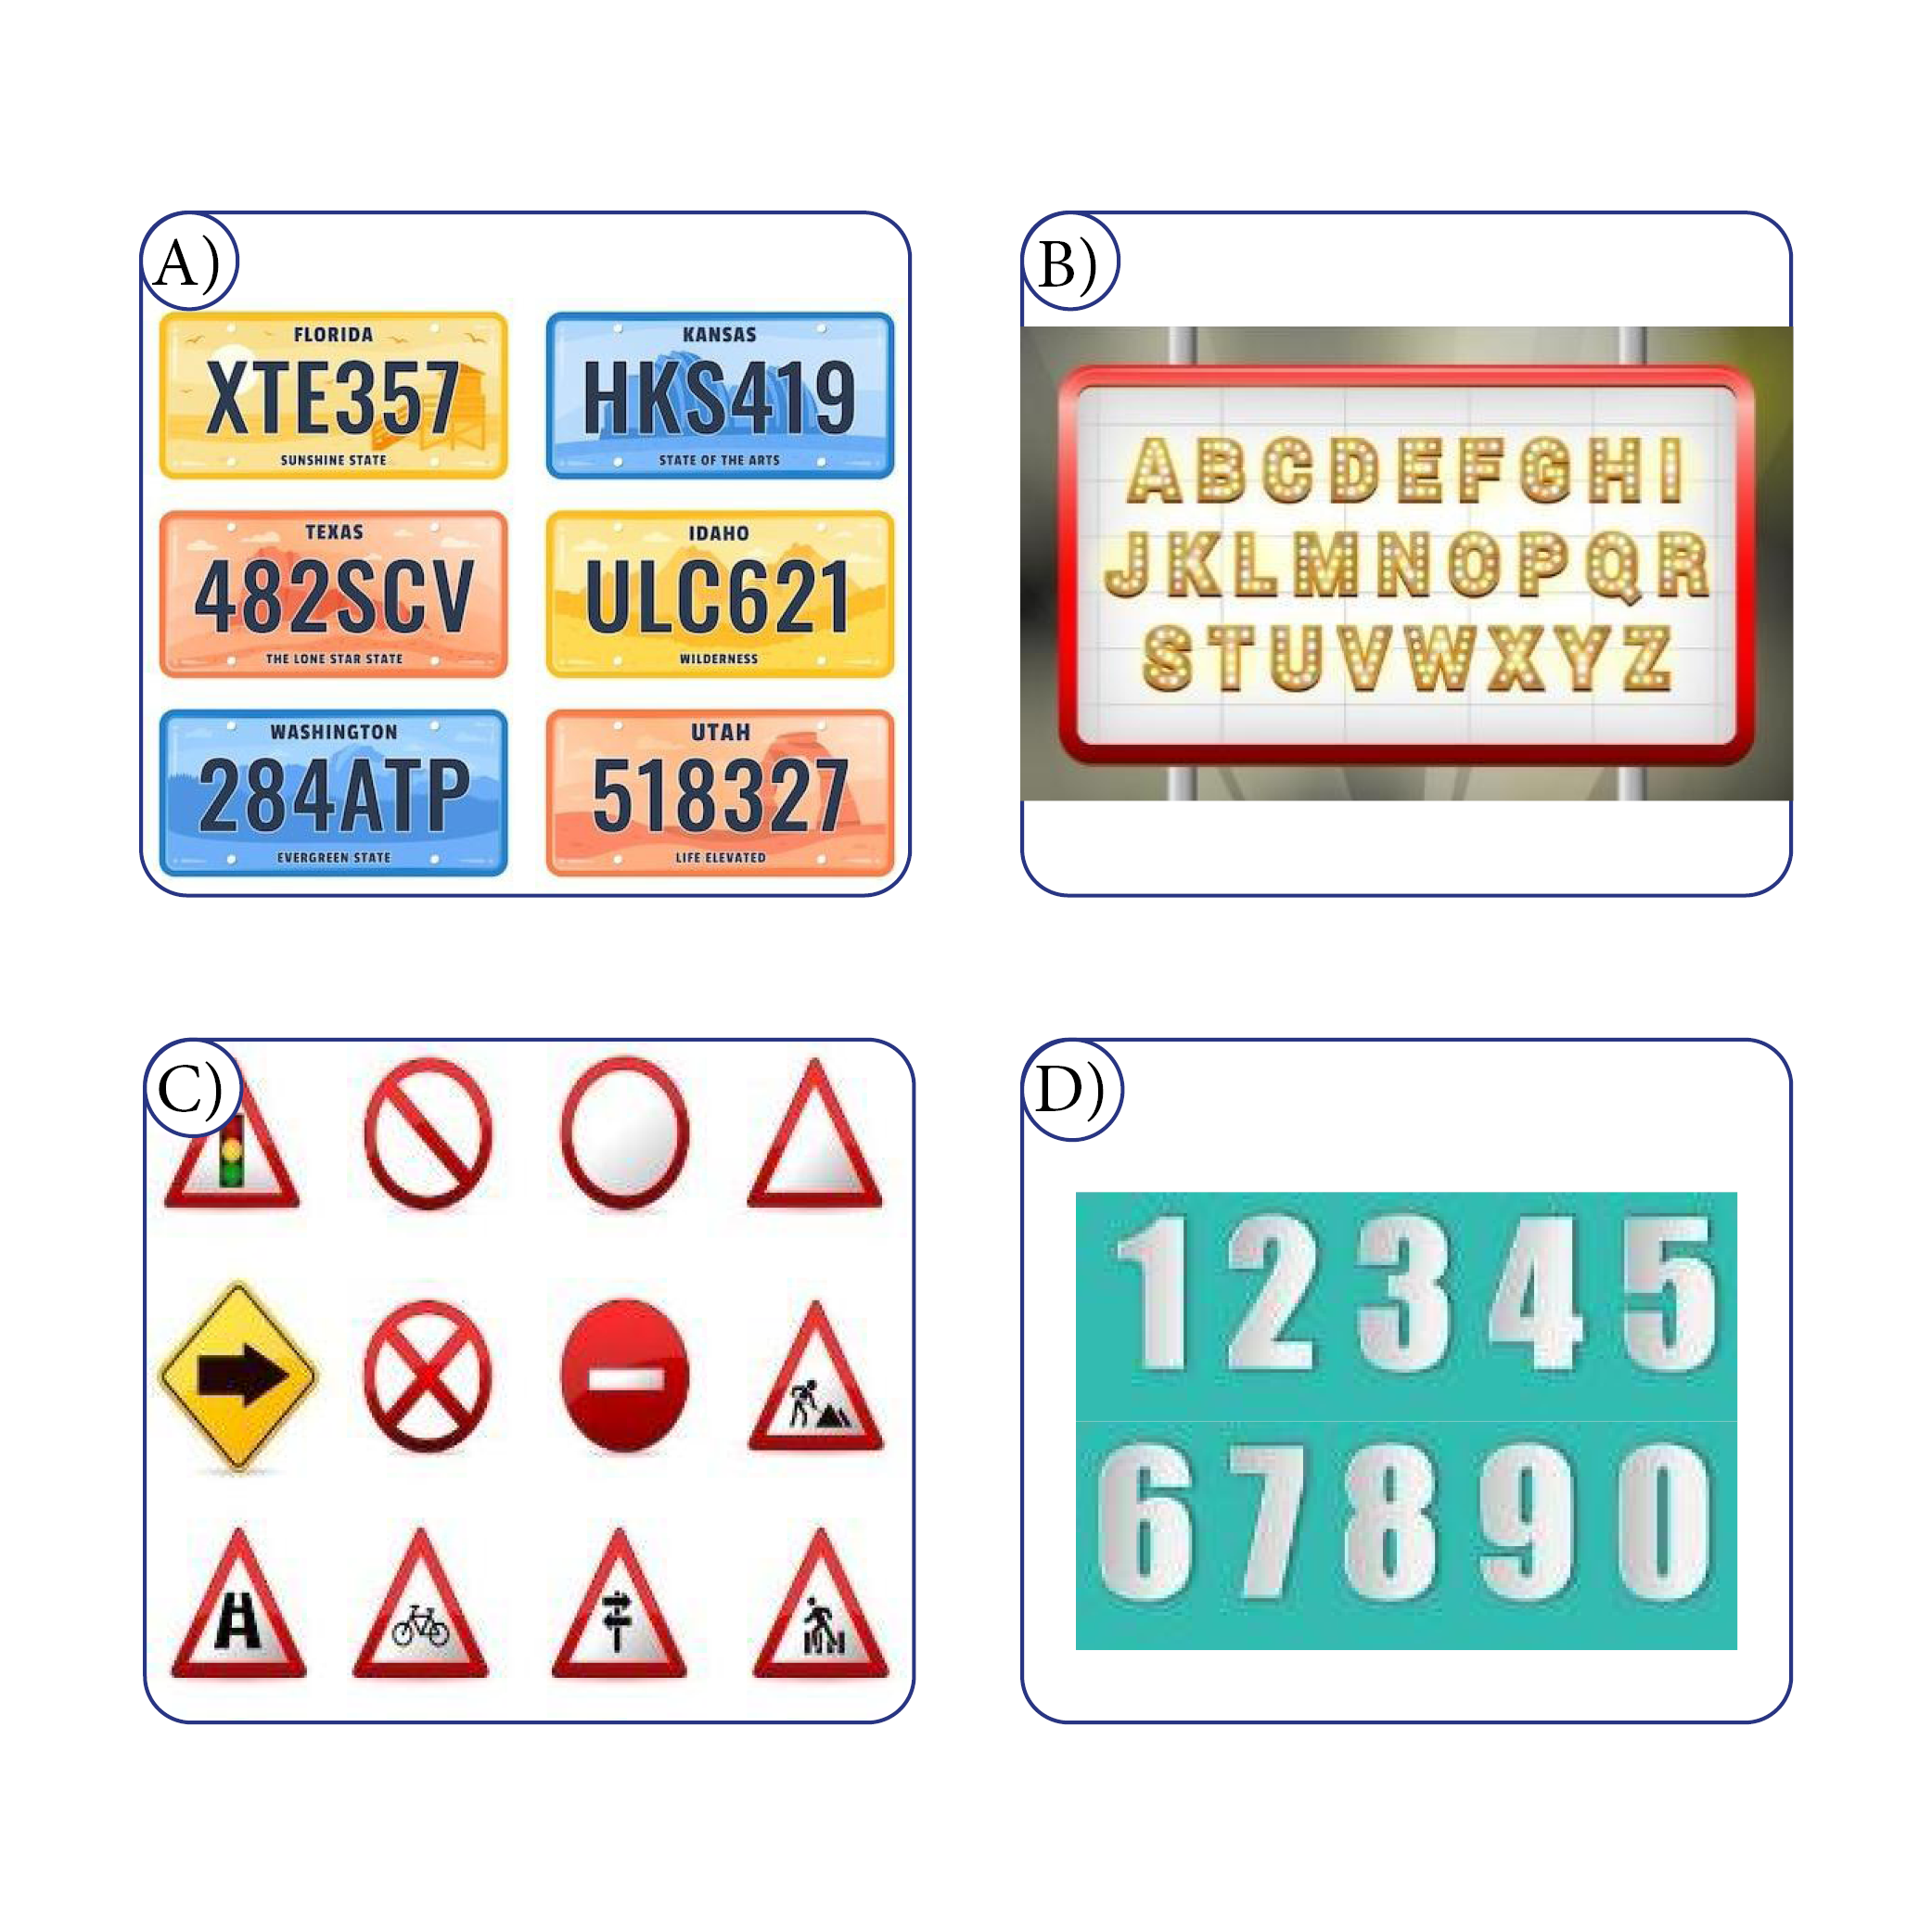
\includegraphics[width=\textwidth]{media/image222a225.png}
\end{figure}

\num{2} MIGUEL ESCOLHEU \textbf{PITOCO} PARA O NOME DE SEU CACHORRO.
QUAL PALAVRA TEM A MESMA QUANTIDADE DE VOGAIS QUE O NOME DO CACHORRO?

\begin{escolha}
\item FADA.

\item CAVALO.

\item TELEVISÃO.

\item GELATINA.
\end{escolha}

\num{3} OBSERVE O DESENHO QUE BIANCA COLORIU.

\begin{figure}[H]
\centering
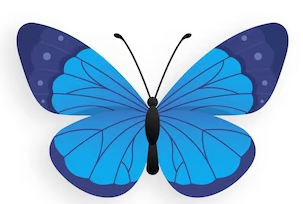
\includegraphics[width=\textwidth]{media/image227.png}
\end{figure}


A PALAVRA QUE TERMINA COM A MESMA SÍLABA QUE O NOME DO ANIMAL DESENHADO É

\begin{multicols}{2}
\begin{escolha}
\item BATATA.

\item TAPETE.

\item BONECA.

\item GILETE.
\end{escolha}
\end{multicols}

\num{4} VEJA A PALAVRA NOVA QUE JOANA ESCREVEU.

\begin{myquote}
\centering\LARGE\textbf{ELEFANTE}
\end{myquote}

% \begin{figure}[H]
% \centering
% 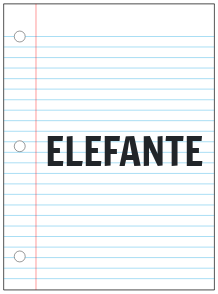
\includegraphics[width=.25\textwidth]{media/image230.png}
% \end{figure}

OS SONS FINAIS QUE FORMAM ESSA PALAVRA SÃO

\begin{multicols}{2}
\begin{escolha}
\item E + E.

\item L + E

\item F + A

\item T + E
\end{escolha}
\end{multicols}

\pagebreak

\num{5} VEJA A PALAVRA QUE UMA MENINA ESCREVEU NA LOUSA.

\begin{myquote}
\centering\LARGE\textbf{CAVALO}
\end{myquote}

A SÍLABA MEDIAL DESSA PALAVRA É

\begin{escolha}
\item CA.

\item VA.

\item LO

\item OL.
\end{escolha}


\num{6} LEIA O TEXTO

\begin{myquote}
\begin{verse}
CARANGUEJO NÃO É PEIXE\\
CARANGUEJO PEIXE É\\
CARANGUEJO SÓ É PEIXE\\
NA ENCHENTE DA MARÉ
\end{verse}

\fonte{DOMÍNIO PÚBLICO.}
\end{myquote}

A ÚLTIMA PALAVRA DO TEXTO É

\begin{escolha}
\item CARANGUEJO.

\item ENCHENTE.

\item PEIXE.

\item MARÉ.
\end{escolha}

\pagebreak

\num{7} LEIA A PALAVRA.

\begin{myquote}
\centering\large{BOLA}
\end{myquote}

A PALAVRA EM QUE NÃO APARECE NENHUMA SÍLABA PERTENCENTE À PALAVRA QUE VOCÊ LEU É 

\begin{escolha}
\item BOLO.

\item LATA.

\item LOBO.

\item FADA.
\end{escolha}


\num{8} VEJA O PRESENTE QUE TALIA DEU PARA SUA AMIGA.

\begin{figure}[H]
\centering

\includegraphics[width=.4\textwidth]{media/image232.png}
\end{figure}

ASSINALE O NOME DO PRESENTE QUE A AMIGA GANHOU.

\begin{multicols}{2}
\begin{escolha}
\item VESTIDO.

\item VETIDO.

\item ETIDO.

\item VETDO.
\end{escolha}
\end{multicols}

\num{9} OBSERVE A IMAGEM.

\begin{figure}[H]
\centering
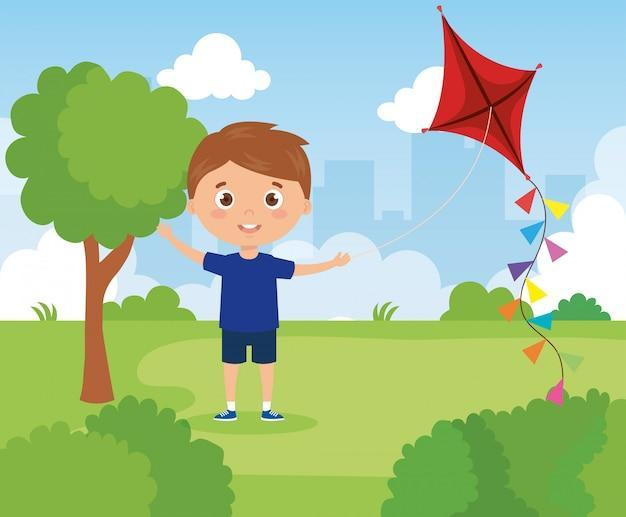
\includegraphics[width=\textwidth]{media/image233.jpg}
\end{figure}

A FRASE QUE REPRESENTA A IMAGEM É

\begin{escolha}[itemsep=-5pt]
\item O MENINO SOBE NA ÁRVORE.

\item O MENINO BRINCA COM A PIPA.

\item O MENINO TOMA BANHO NO RIO.

\item O MENINO SE ESCONDE ATRÁS DO ARBUSTO.
\end{escolha}

\conteudo{LEMBRE-SE: LER IMAGENS TAMBÉM É UM TIPO DE LEITURA DE TEXTO.}

\num{10} VEJA O ANIMAL PREFERIDO DE BRUNO.

\begin{figure}[H]
\centering
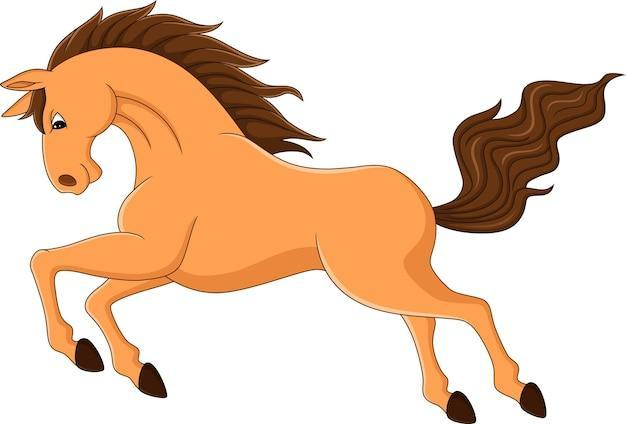
\includegraphics[width=\textwidth]{media/image234.jpg}
\end{figure}


O NOME CORRETO DESSE ANIMAL É

%\begin{multicols}{2}
\begin{escolha}
\item VALO.

\item KAVA.

\item CAVALO.

\item VALOCA.
\end{escolha}
%\end{multicols}

\conteudo{NA QUESTÃO DE NÚMERO 10, PARA ENCONTRAR A PALAVRA CORRETA, TENTE SE LEMBRAR DA PRIMEIRA LETRA DO NOME DO ANIMAL E DA QUANTIDADE DE SÍLABAS QUE ESSA PALAVRA TEM.}

\num{11} OBSERVE O MÓVEL QUE CARLA COMPROU.

\begin{figure}[H]
\centering
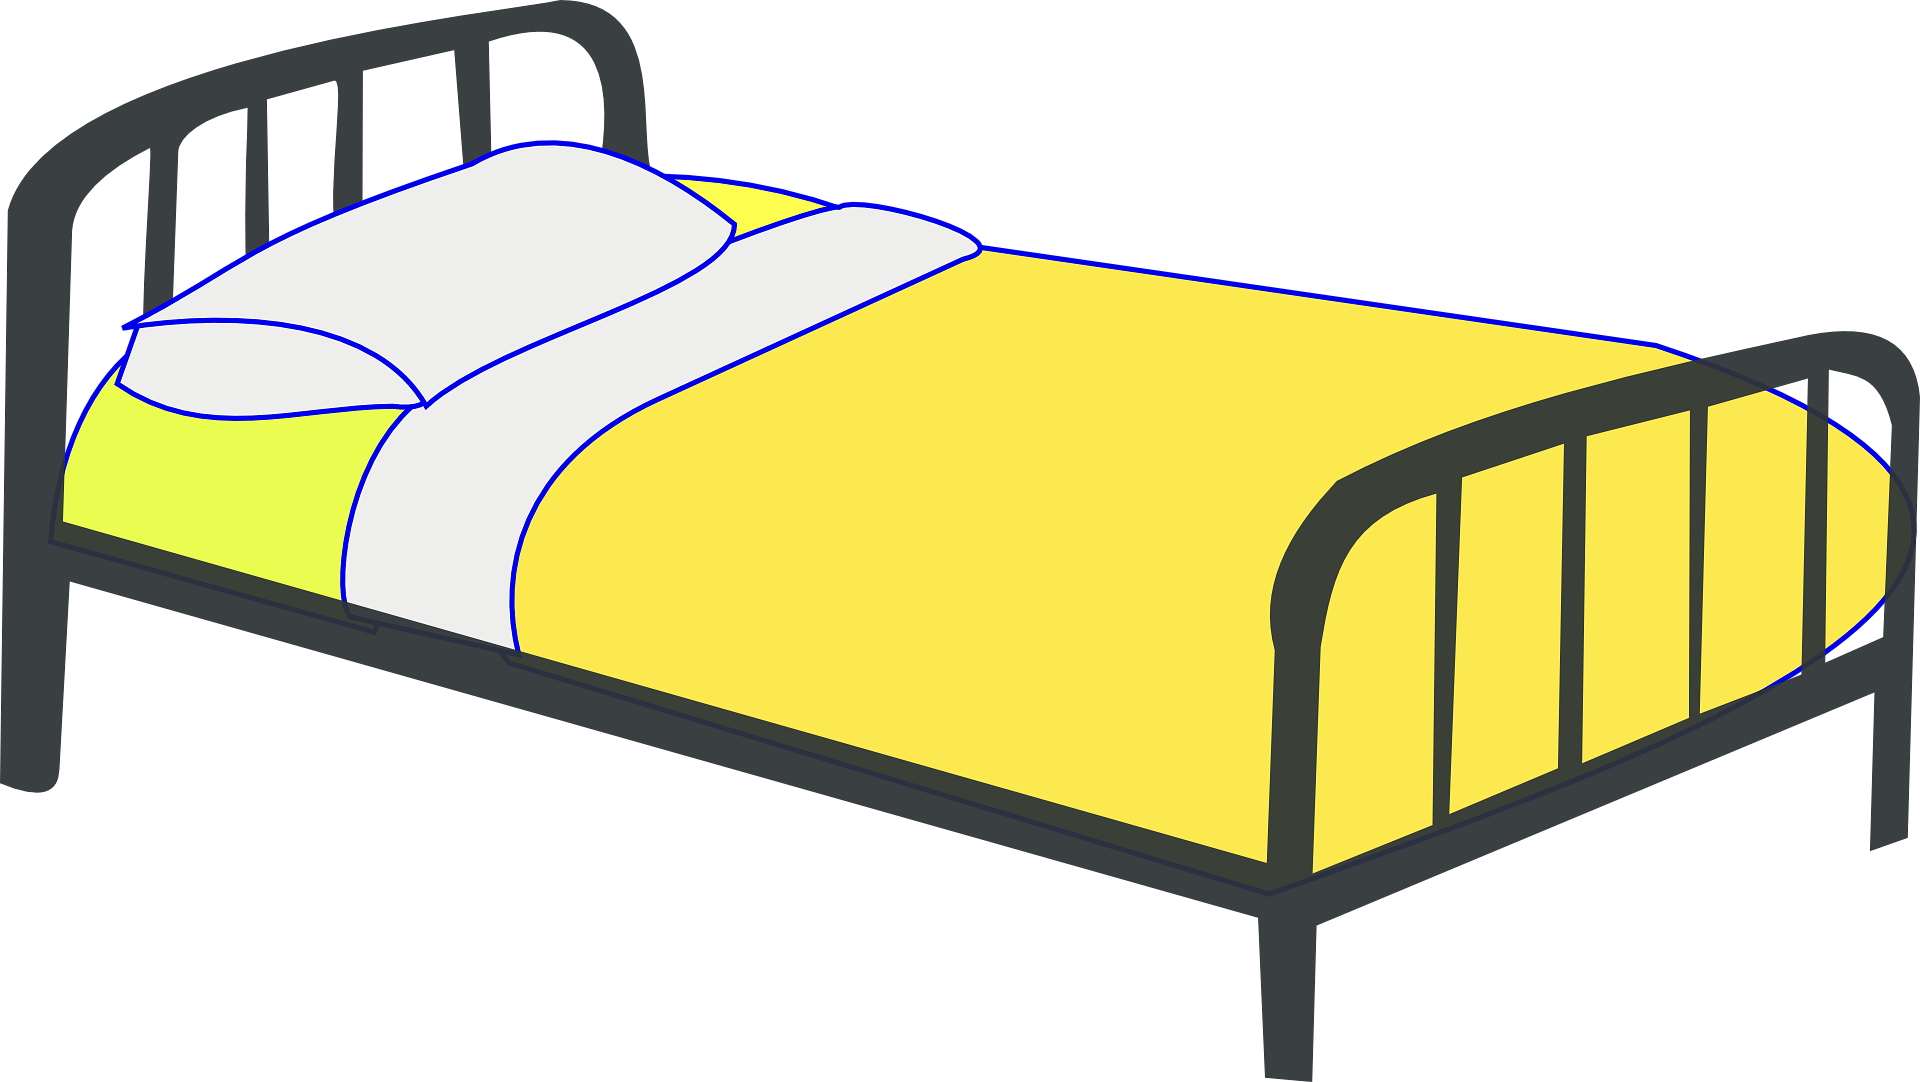
\includegraphics[width=.65\textwidth]{media/image235a.png}
\end{figure}

A PALAVRA QUE COMEÇA COM A MESMA SÍLABA FINAL QUE O NOME DO MÓVEL DE CARLA É 

\begin{multicols}{2}
\begin{escolha}[itemsep=0pt]
\item CANELA.

\item BONECA.

\item SACADA.

\item MACACO.
\end{escolha}
\end{multicols}

\num{12} LEIA O TEXTO.

\begin{myquote}
\begin{verse}
SAPO CURURU\\
DA BEIRA DO RIO\\
QUANDO O SAPO GRITA\\
OH! MANINHA\\
É PORQUE TEM FRIO.
\end{verse}

\fonte{DOMÍNIO PÚBLICO.}
\end{myquote}

POR QUE O SAPO GRITOU?

\begin{escolha}[itemsep=0pt]
\item PORQUE ESTÁ ASSUSTADO. 

\item PORQUE ESTÁ COM FRIO.

\item PORQUE ESTÁ BRINCANDO.

\item PORQUE QUER ASSUSTAR SEUS AMIGOS.
\end{escolha}

\pagebreak

\num{13} LEIA A LISTA.

\begin{myquote}
\begin{enumerate}
\item ARROZ

\item FEIJÃO

\item MACARRÃO

\item ÓLEO

\item BISCOITO

% \item EXTRATO DE TOMATE

% \item FARINHA DE TRIGO

% \item LEITE
\end{enumerate}
\end{myquote}

ESSE TEXTO SERVE PARA

\begin{escolha}
\item ORGANIZAR TAREFAS.

\item ENSINAR A FAZER UM PRATO.

\item INDICAR OS PRODUTOS.

\item DIVULGAR UM EVENTO.
\end{escolha}

\begin{figure}[H]
\centering
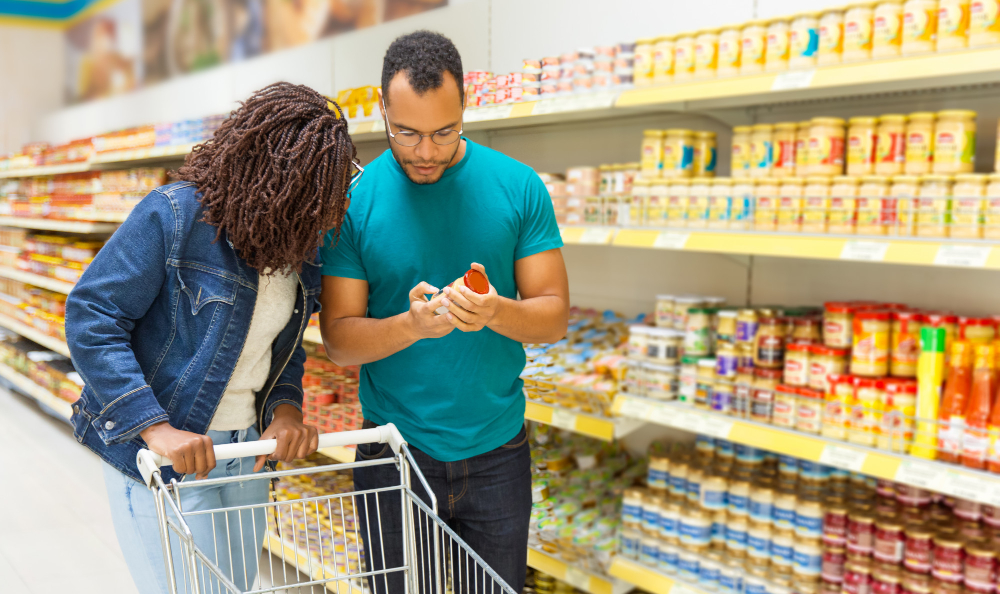
\includegraphics[width=\textwidth]{media/image273.png}
\end{figure}

\pagebreak

\num{14} LEIA O TEXTO. \enlargethispage{2\baselineskip}

\begin{myquote}
\begin{verse}
\textbf{TEREZINHA DE JESUS}

TEREZINHA DE JESUS\\
DE UMA QUEDA FOI AO CHÃO\\
ACUDIRAM TRÊS CAVALHEIROS\\
TODOS TRÊS, CHAPÉU NA MÃO.
\end{verse}

\vspace{1cm}

\begin{center}
\includegraphics[width=\textwidth]{media/image274.png}
\end{center}

\vspace{1cm}

\begin{verse}
O PRIMEIRO, FOI SEU PAI\\
O SEGUNDO, SEU IRMÃO\\
O TERCEIRO FOI AQUELE\\
A QUE TEREZA DEU A MÃO.
\end{verse}

\fonte{DOMÍNIO PÚBLICO.}
\end{myquote}

DE QUE O TEXTO FALA?

\begin{escolha}%[itemsep=-5pt]
\item DO PAI DE TEREZINHA.

\item DA MÃO DE TEREZINHA.

\item DO IRMÃO DE TEREZINHA.

\item DA QUEDA DE TEREZINHA.
\end{escolha}

\pagebreak

\num{15} LEIA O TEXTO. \enlargethispage{2\baselineskip}

\begin{myquote}
\textbf{A RAPOSA E O CORVO}

\uppercase{O corvo conseguiu arranjar um pedaço de queijo. Saiu voando, com o queijo no bico, até pousar numa
árvore.

Quando viu o queijo, a raposa resolveu se apoderar
dele. Chegou ao pé da árvore e começou a bajular o corvo:}

\begin{center}
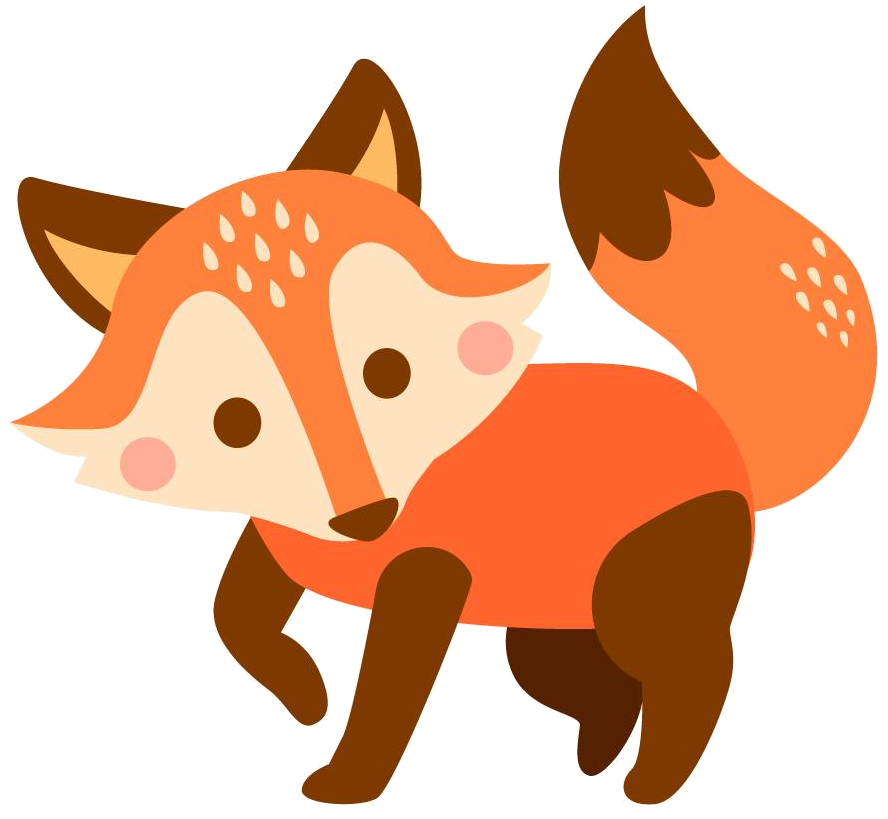
\includegraphics[width=.3\textwidth]{media/image275.png}
\end{center}

\uppercase{--- O senhor é certamente o mais belo
dos animais! Se souber cantar tão bem quanto a sua plumagem
é linda, não haverá ave que possa se comparar.

Acreditando nos elogios, o corvo pôs-se imediatamente
a cantar. Mas, ao abrir o bico, deixou
cair o queijo.

A raposa abocanhou o queijo e foi
embora.}

\fonte{CONTOS TRADICIONAIS, FÁBULAS, LENDAS E MITOS. MINISTÉRIO DA EDUCAÇÃO. BRASÍLIA: FUNDESCOLA, 2000. P. 105.}
\end{myquote}

A RAPOSA QUERIA QUE O CORVO CANTASSE PARA

\begin{multicols}{2}
\begin{escolha}[itemsep=0pt]
\item ALEGRAR A FLORESTA.

\item MOSTRAR TALENTO.

\item GANHAR ELOGIOS.

\item PEGAR O QUEIJO.
\end{escolha}
\end{multicols}

\pagebreak

\num{16} LEIA A TIRINHA.

\begin{figure}[H]
\includegraphics[width=\textwidth]{media/image236a238.png}
% 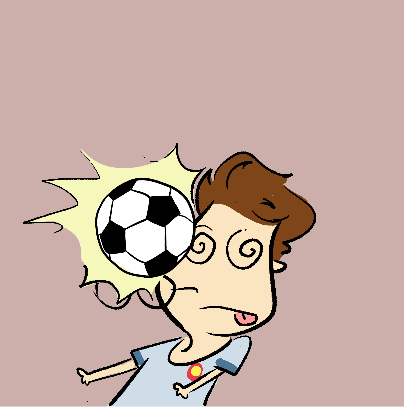
\includegraphics[width=1.92708in,height=1.92708in]{media/image237.png}
% 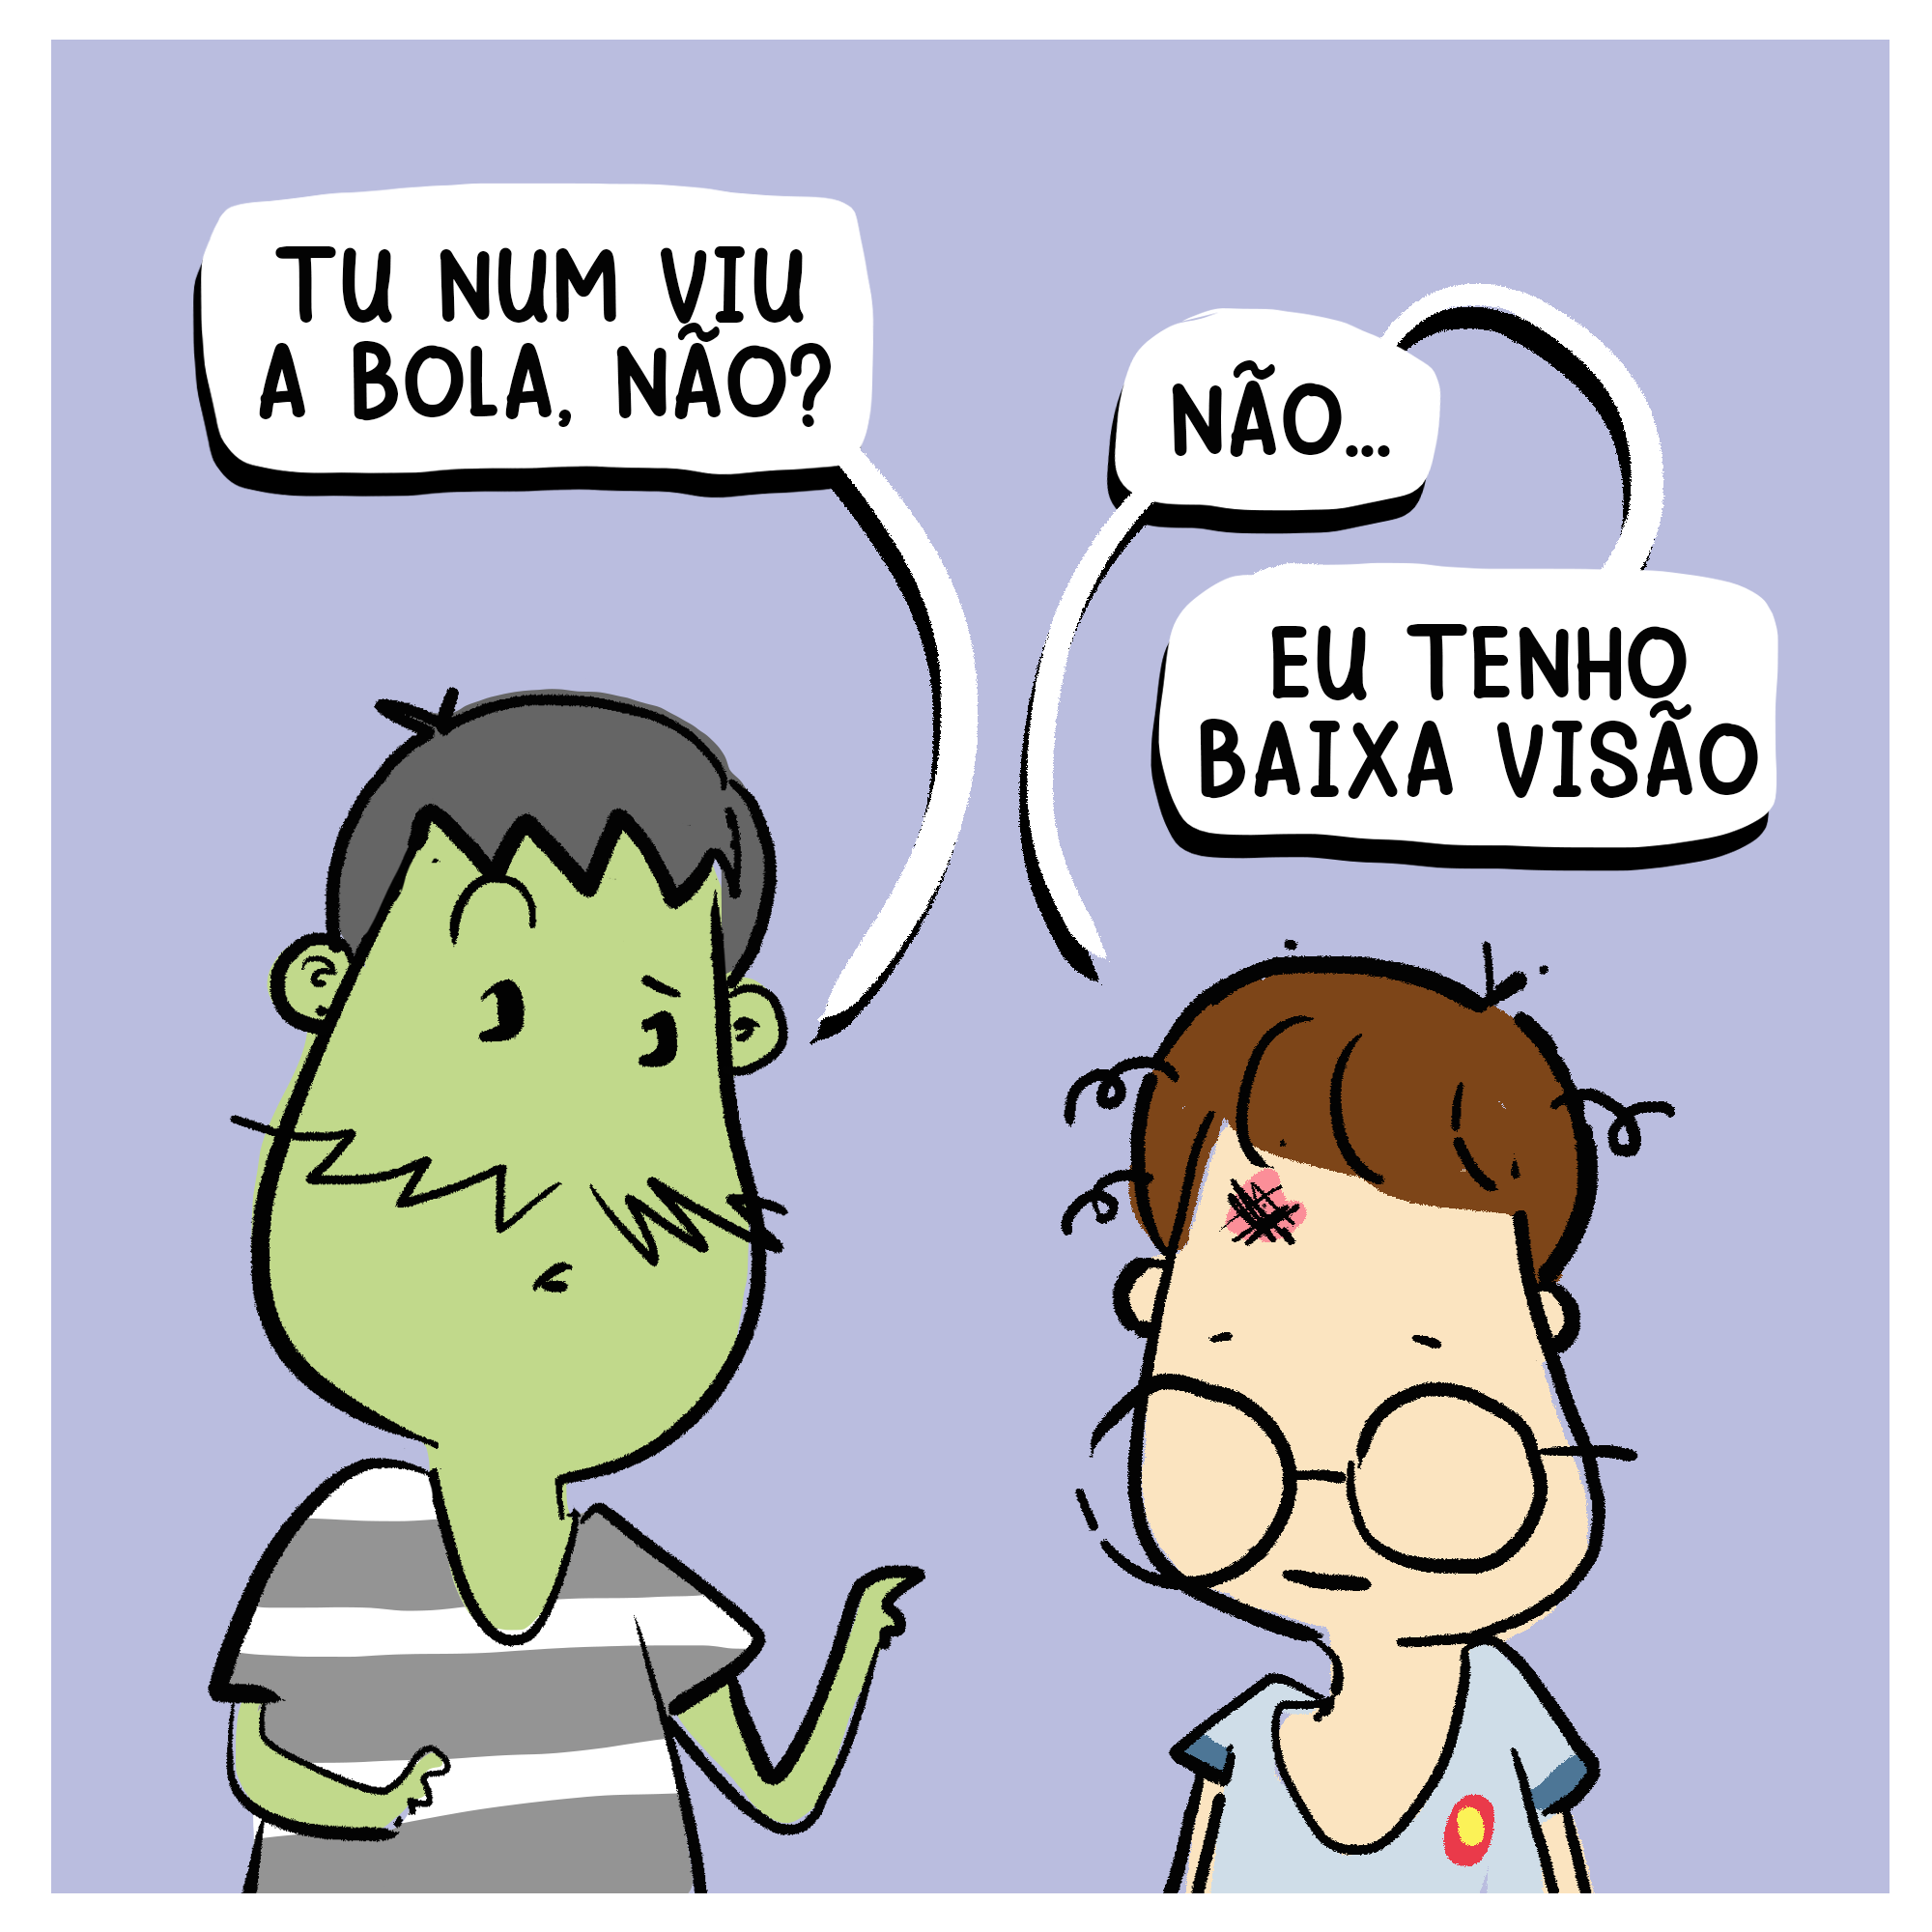
\includegraphics[width=1.90625in,height=1.90625in]{media/image238.png}
\end{figure}

%Disponível em https://lizeseusamigos.org.br/tirinhas/tirinhas-tres. Acesso 20 Fev 2023.

A BOLA ACERTOU JUNINHO NO SEGUNDO QUADRINHO PORQUE ELE

\begin{escolha}
\item É MUITO DISTRAÍDO.

\item TENTOU PEGAR A BOLA. 

\item ESTAVA JOGANDO COMO GOLEIRO.

\item TEM DIFICULDADE DE ENXERGAR.
\end{escolha}

\chapter[Simulado 4]{Simulado}
\markboth{Simulado 4}{}

\pagebreak

\num{1} BIA QUER MOSTRAR O NOME QUE ESCOLHEU PARA SUA BONECA.
A PLACA QUE ELA VAI ESCOLHER PARA FORMAR O NOME É

\begin{figure}[H]
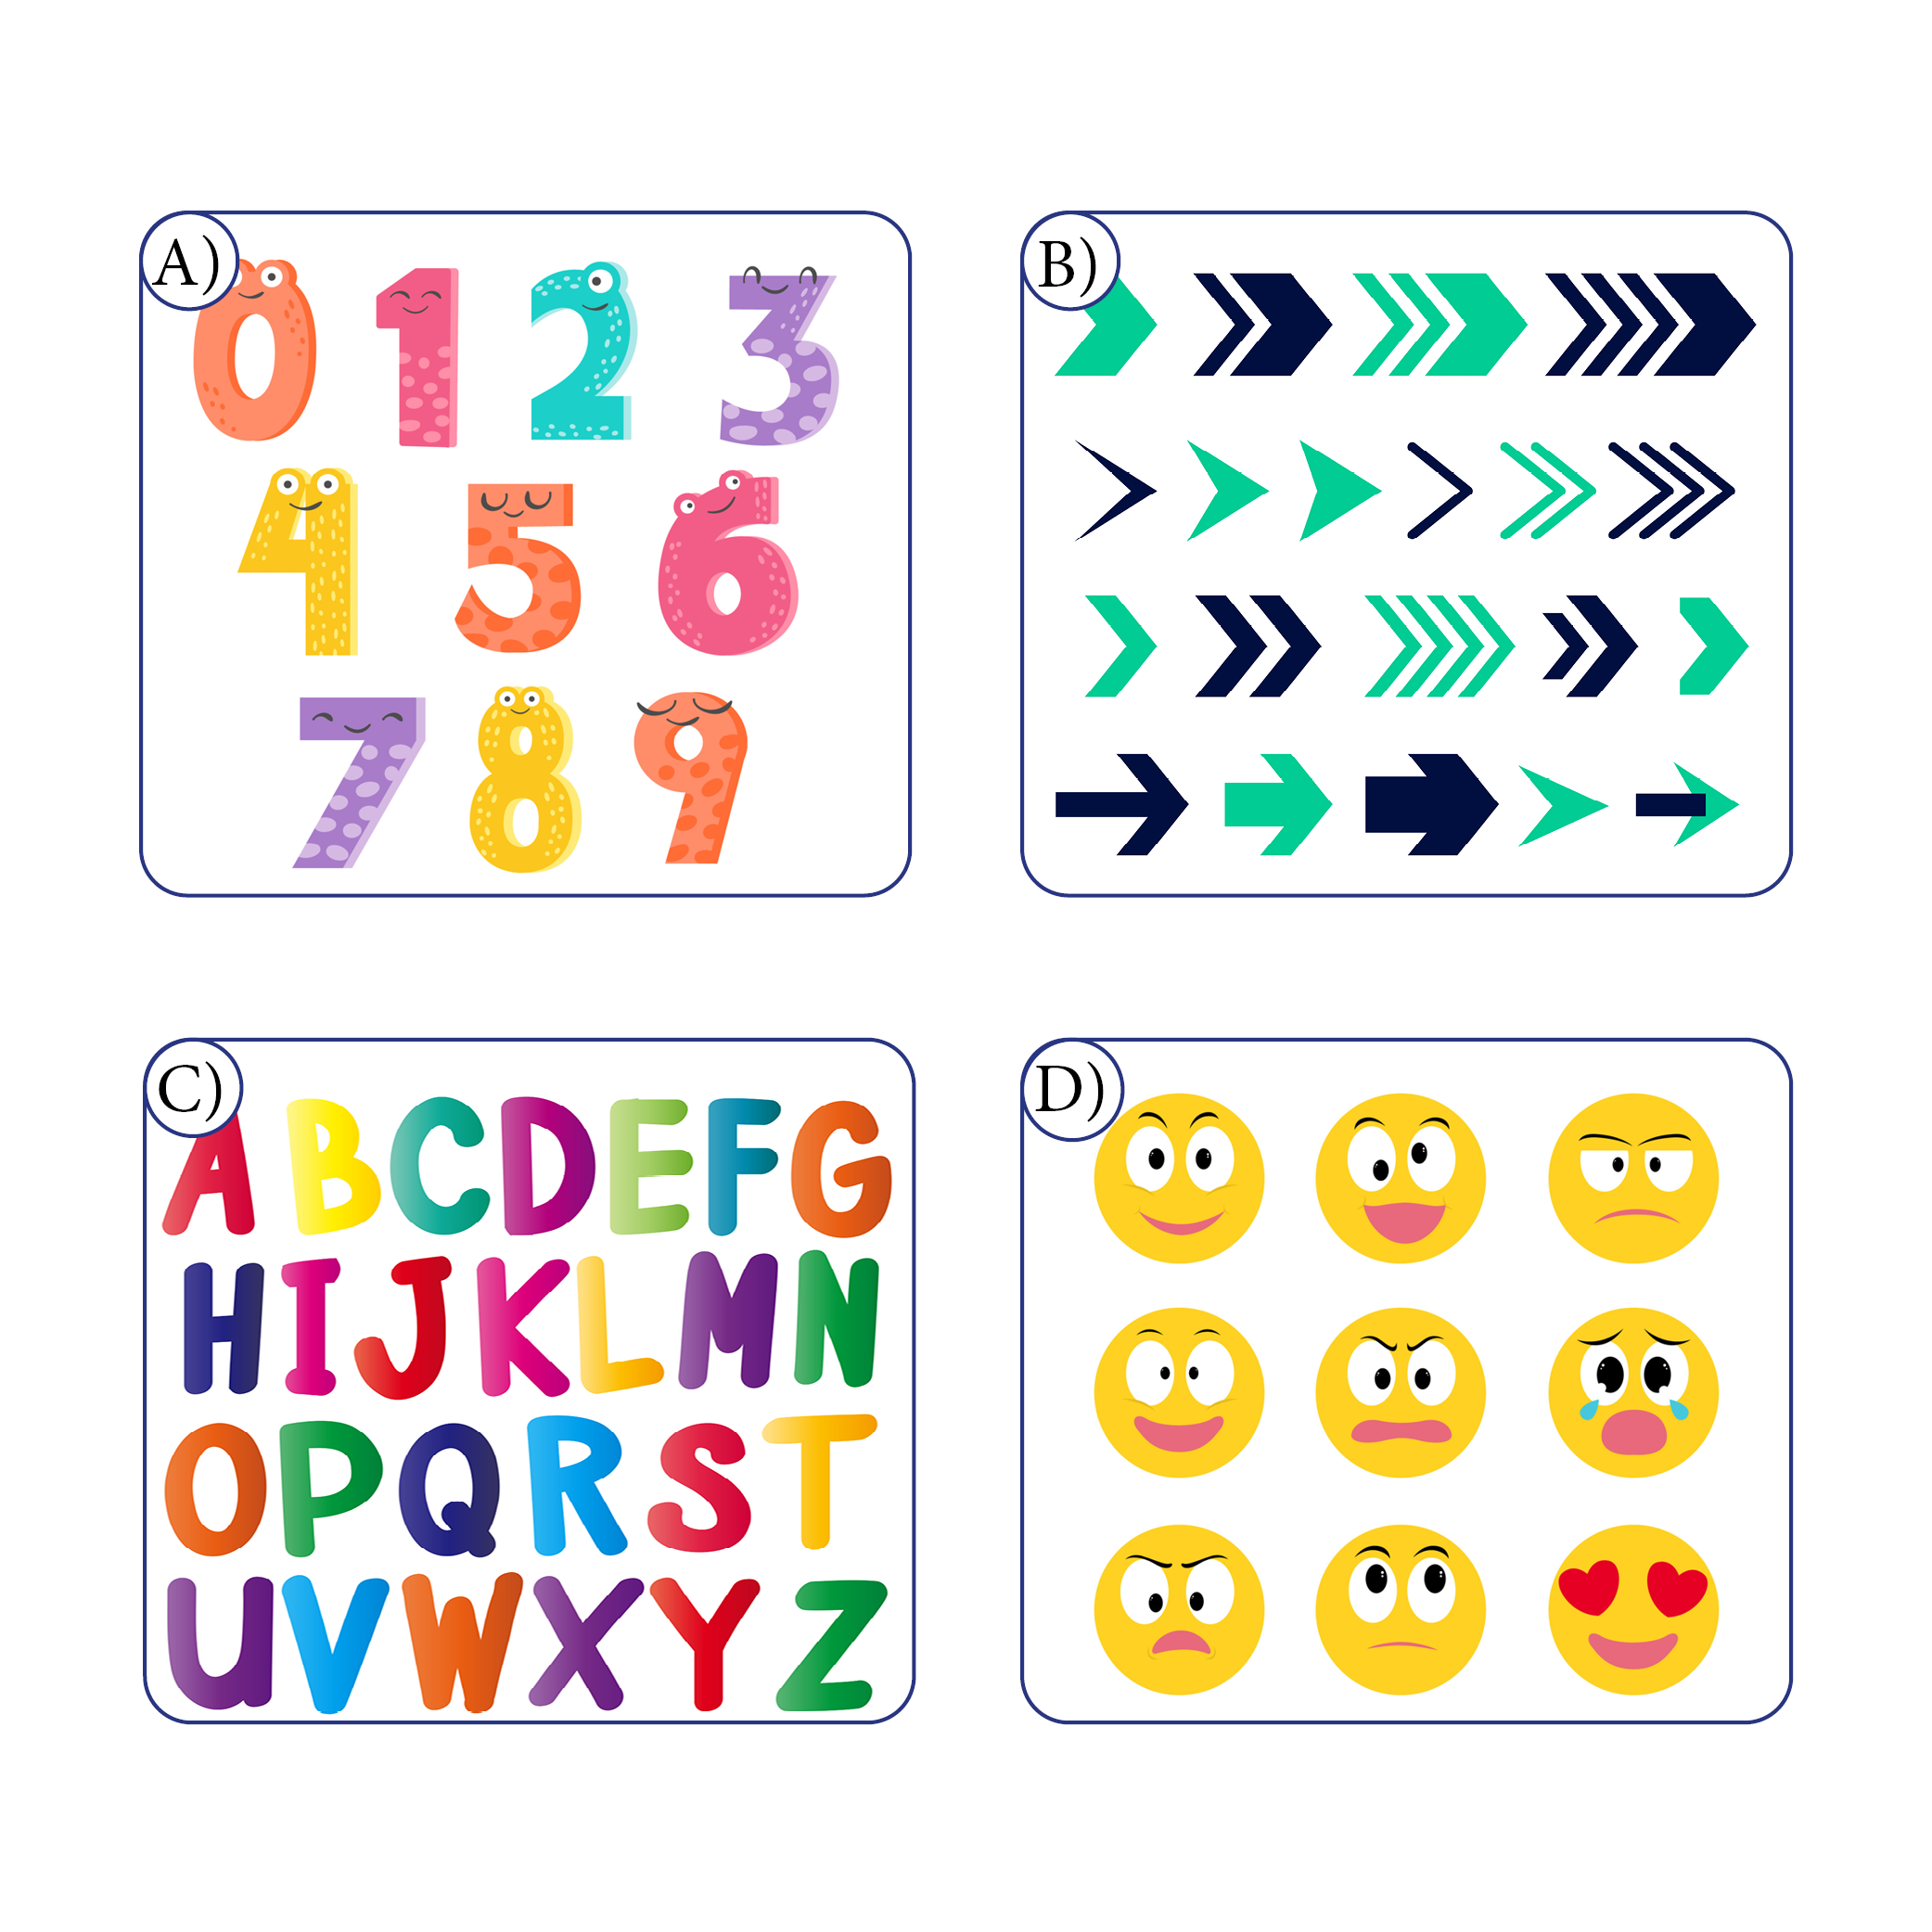
\includegraphics[width=\textwidth]{media/image239a242.png}
\end{figure}

\conteudo{PARA A QUESTÃO DE NÚMERO 1, PENSE NO TIPO DE SÍMBOLO DE QUE BIA PRECISA PARA ESCREVER O NOME DE SUA BONECA. ENCONTRE ESSES SÍMBOLOS ENTRE OS QUATRO AGRUPAMENTOS.}

\pagebreak

\num{2} VEJA A PALAVRA QUE MARIA ESCREVEU.

\begin{myquote}
\centering\Large\textbf{SALADA}
\end{myquote}

AS LETRAS QUE FORMAM O SOM FINAL DA PALAVRA SÃO

\begin{multicols}{2}
\begin{escolha}
\item D + A.

\item L + A.

\item S + A.

\item A + D.
\end{escolha}
\end{multicols}

\num{3} VEJA A PALAVRA QUE DINO CONSEGUIU ESCREVER.

\begin{myquote}
\centering\Large\textbf{BORBOLETA}
\end{myquote}

A PALAVRA QUE TEM A MESMA QUANTIDADE DE SONS QUE ESSA PALAVRA É 

\begin{multicols}{2}
\begin{escolha}%[itemsep=0pt]
\item BICICLETA.

\item PATINETE.

\item PATINS.

\item BONÉ.
\end{escolha}
\end{multicols}

\num{4} VEJA A PALAVRA QUE ISA ENCONTROU NO SEU LIVRO. 

\begin{myquote}
\centering\Large\textbf{JANELA}
\end{myquote}

A PALAVRA QUE TEM A MESMA SÍLABA INICIAL QUE A PALAVRA QUE ISA ENCONTROU É

\begin{multicols}{2}
\begin{escolha}%[itemsep=0pt]
\item NEVE.

\item JACARÉ.

\item PANELA.

\item LARANJA.
\end{escolha}
\end{multicols}

\pagebreak

\num{5} VEJA O BRINQUEDO QUE ENZO GANHOU.

\begin{figure}[H]
\centering
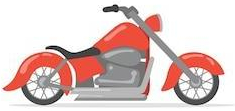
\includegraphics[width=.6\textwidth]{media/image245.jpg}
\end{figure}

%https://www.freepik.com/vectors/motorcycle\#referrer=detail\&resource=11672041

A PALAVRA QUE NÃO APRESENTA NENHUM DOS SONS DO NOME DO BRINQUEDO DE ENZO É

\begin{multicols}{2}
\begin{escolha}
\item FADA.

\item GATO.

\item MOLA.

\item RATO.
\end{escolha}
\end{multicols}

\num{6} LEIA A ADIVINHA. 

\begin{myquote}
\begin{verse}
COM DEZ PATAS VAI DE LADO,\\
CONSTELAÇÃO TEM SEU NOME,\\
NÃO TEM PESCOÇO E É CAÇADO\\
PORQUE É GOSTOSO E SE COME.
\end{verse}

\fonte{DOMÍNIO PÚBLICO.}
\end{myquote}

A PRIMEIRA PALAVRA DESSE TEXTO É

\begin{escolha}
\item COM.

\item LADO.

\item COME.

\item PORQUE.
\end{escolha}


\num{7} OBSERVE O ANIMAL DE ESTIMAÇÃO QUE LETÍCIA GANHOU.

\begin{figure}[H]
\centering
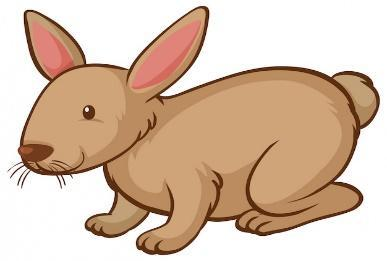
\includegraphics[width=.6\textwidth]{media/image246.jpg}
\end{figure}

O NOME CORRETO DESSE ANIMAL É

\begin{escolha}
\item LHOECO.

\item COOLHO.

\item EOCLHO.

\item COELHO.
\end{escolha}

\num{8} LEIA A PALAVRA QUE CATARINA ESCREVEU.

\begin{myquote}
\centering\Large\textbf{MACACO}
\end{myquote}

A PALAVRA QUE COMEÇA COM O SOM IGUAL À PALAVRA QUE ELA ESCREVEU É 

%\begin{multicols}{2}
\begin{escolha}
\item NABO.

\item CANECA.

\item COCADA.

\item MACARRÃO.
\end{escolha}
%\end{multicols}

\num{9} SARA GANHOU UM \textbf{TELE\_\_NE} DE SUA TIA. ASSINALE A SÍLABA QUE COMPLETA CORRETAMENTE A PALAVRA.

\begin{multicols}{2}
\begin{escolha}
\item CO.

\item PA.

\item FO.

\item FA.
\end{escolha}
\end{multicols}

\num{10} LEIA A FRASE A SEGUIR.

\begin{myquote}
\centering\large\textbf{OS PATOS NADAM NO LAGO.}
\end{myquote}

QUAL DESENHO REPRESENTA ESSA FRASE?

\begin{multicols}{2}
\begin{escolha}
\item 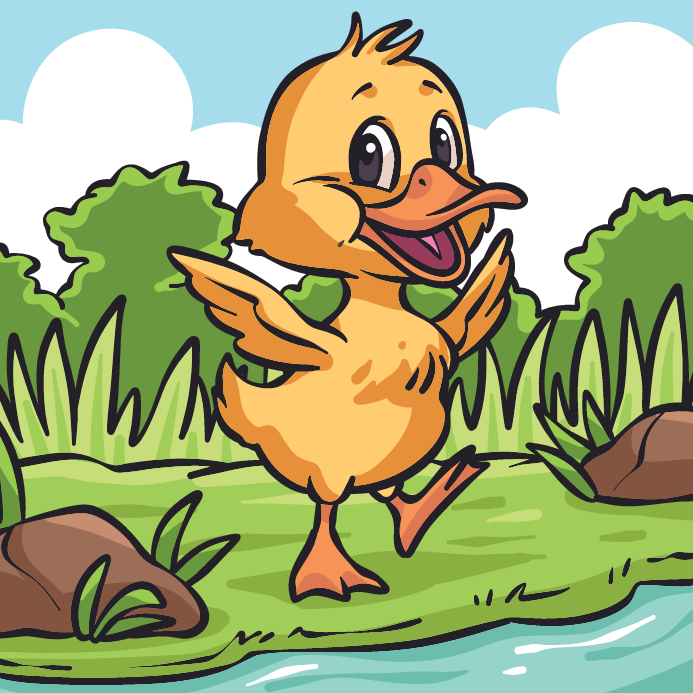
\includegraphics[width=.4\textwidth]{media/image250.png}

\item 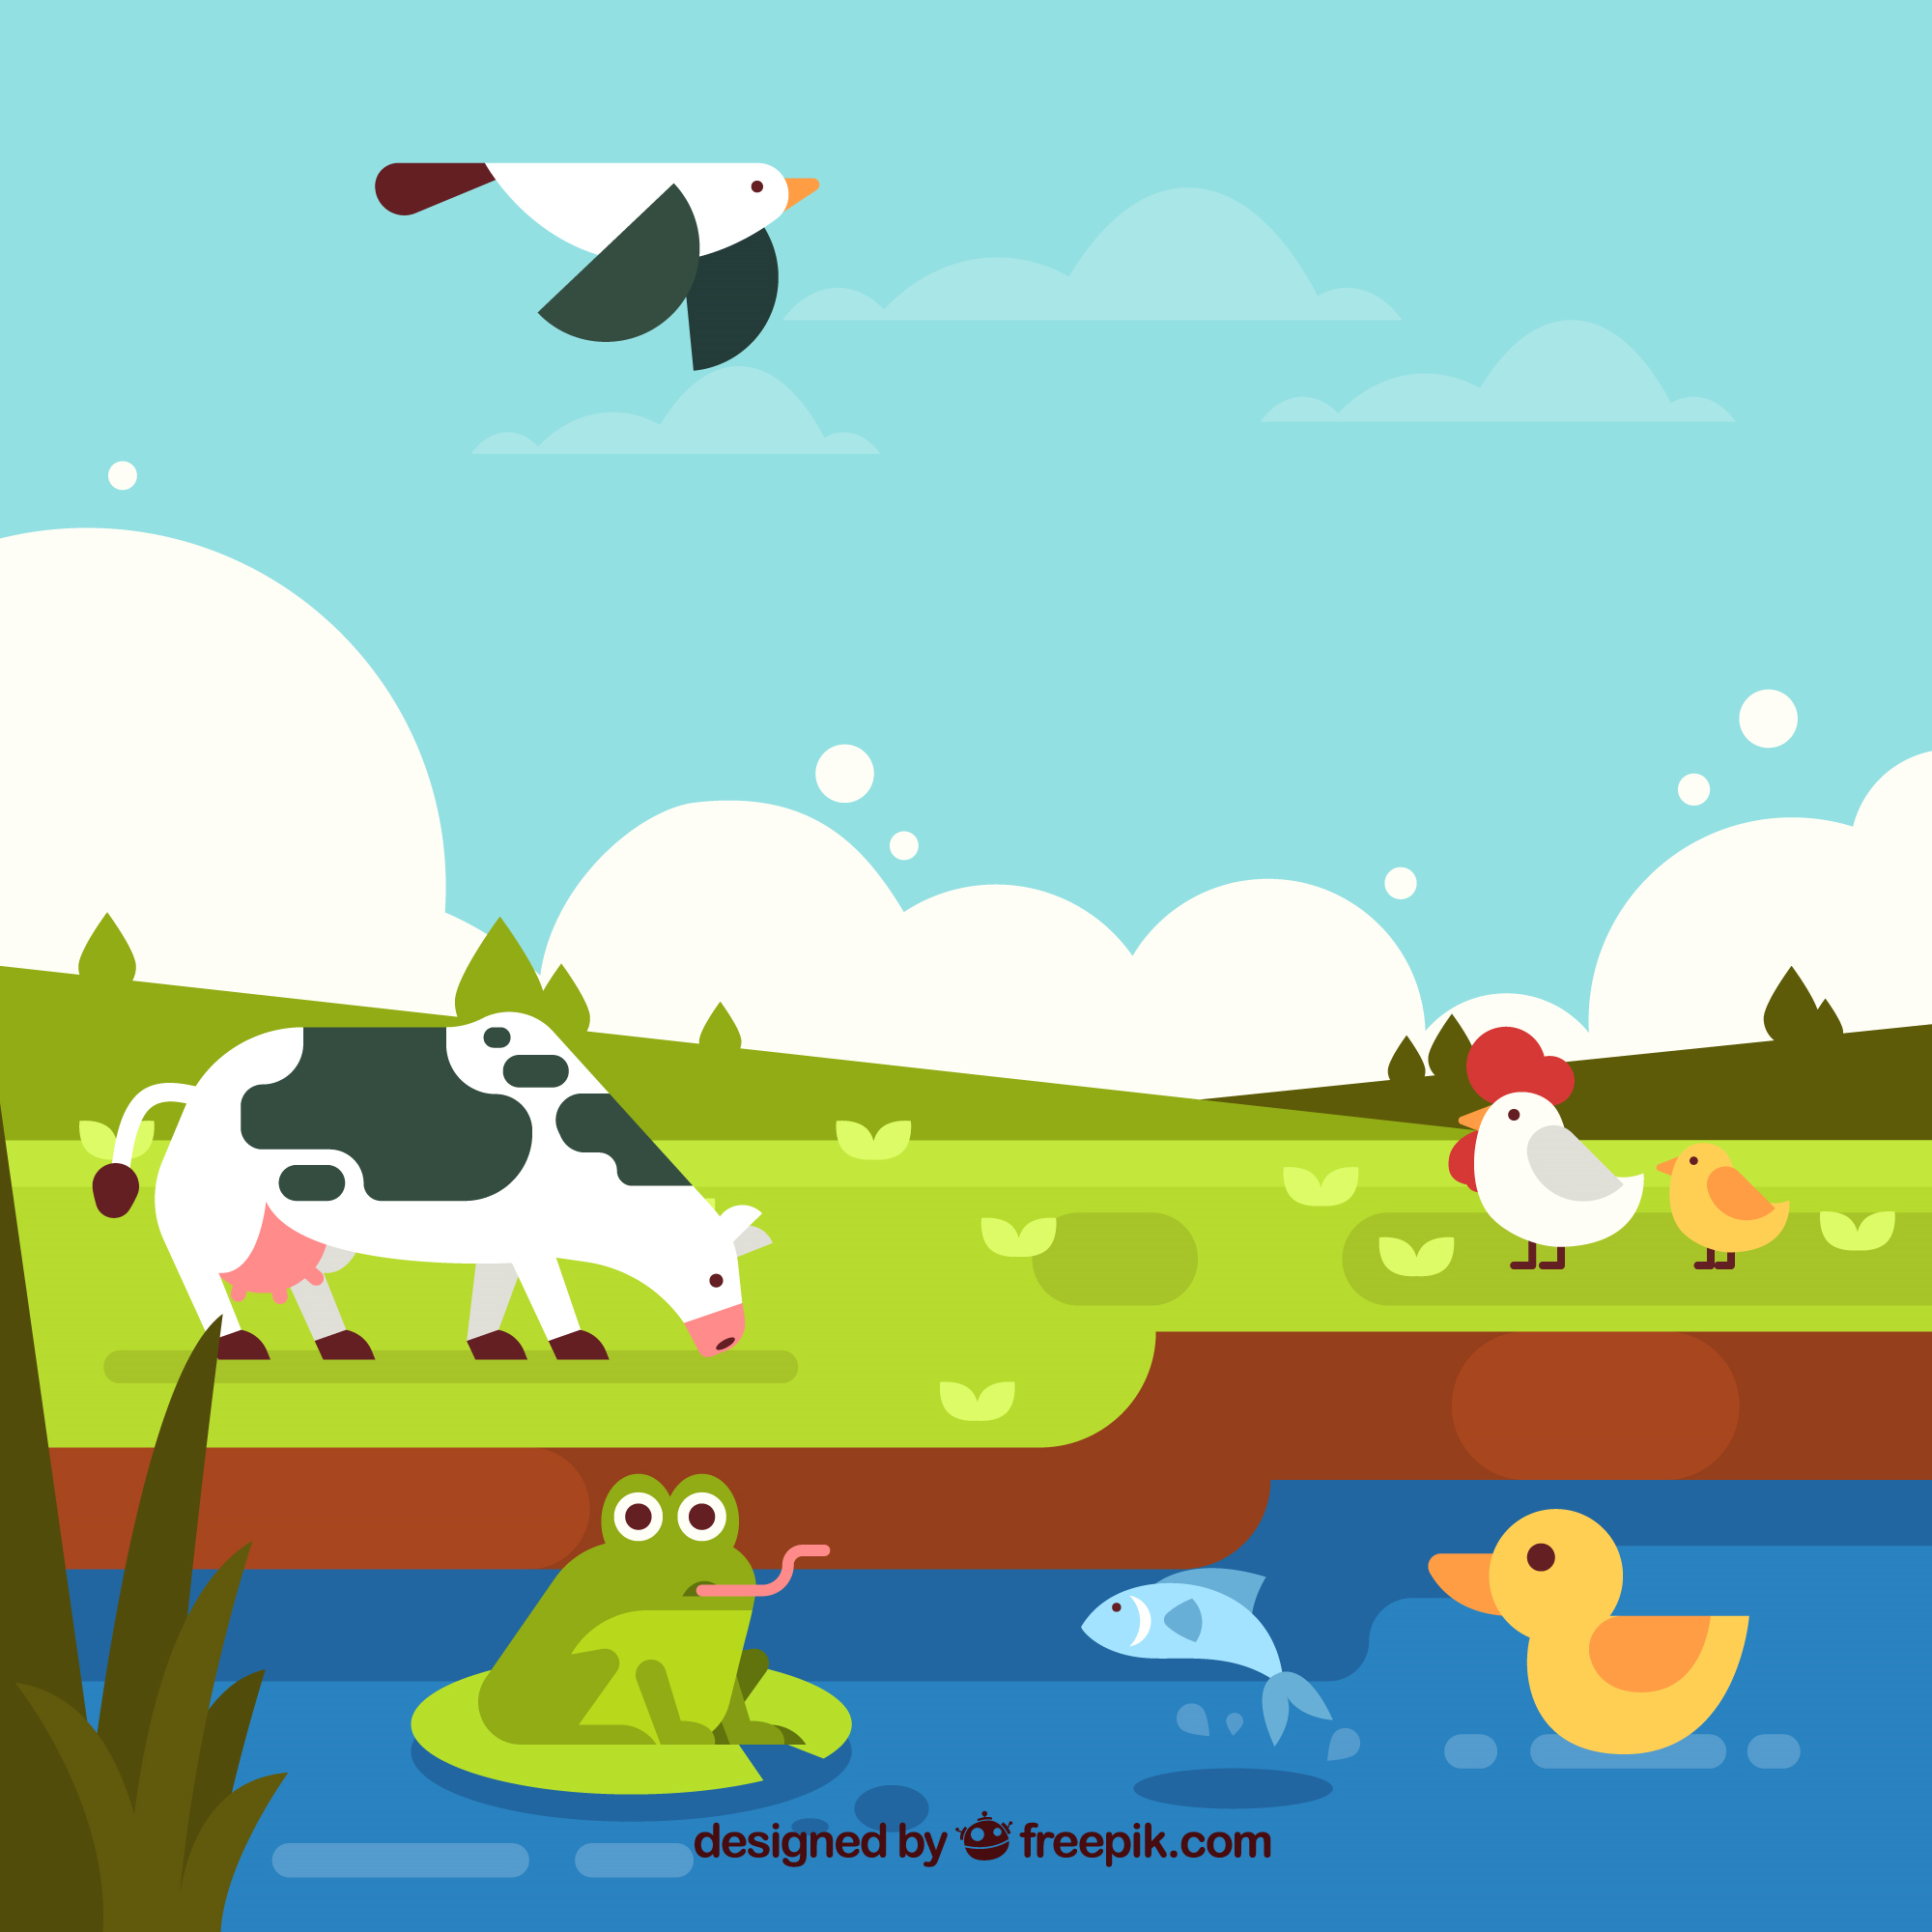
\includegraphics[width=.4\textwidth]{media/image251.png}

\columnbreak

\item 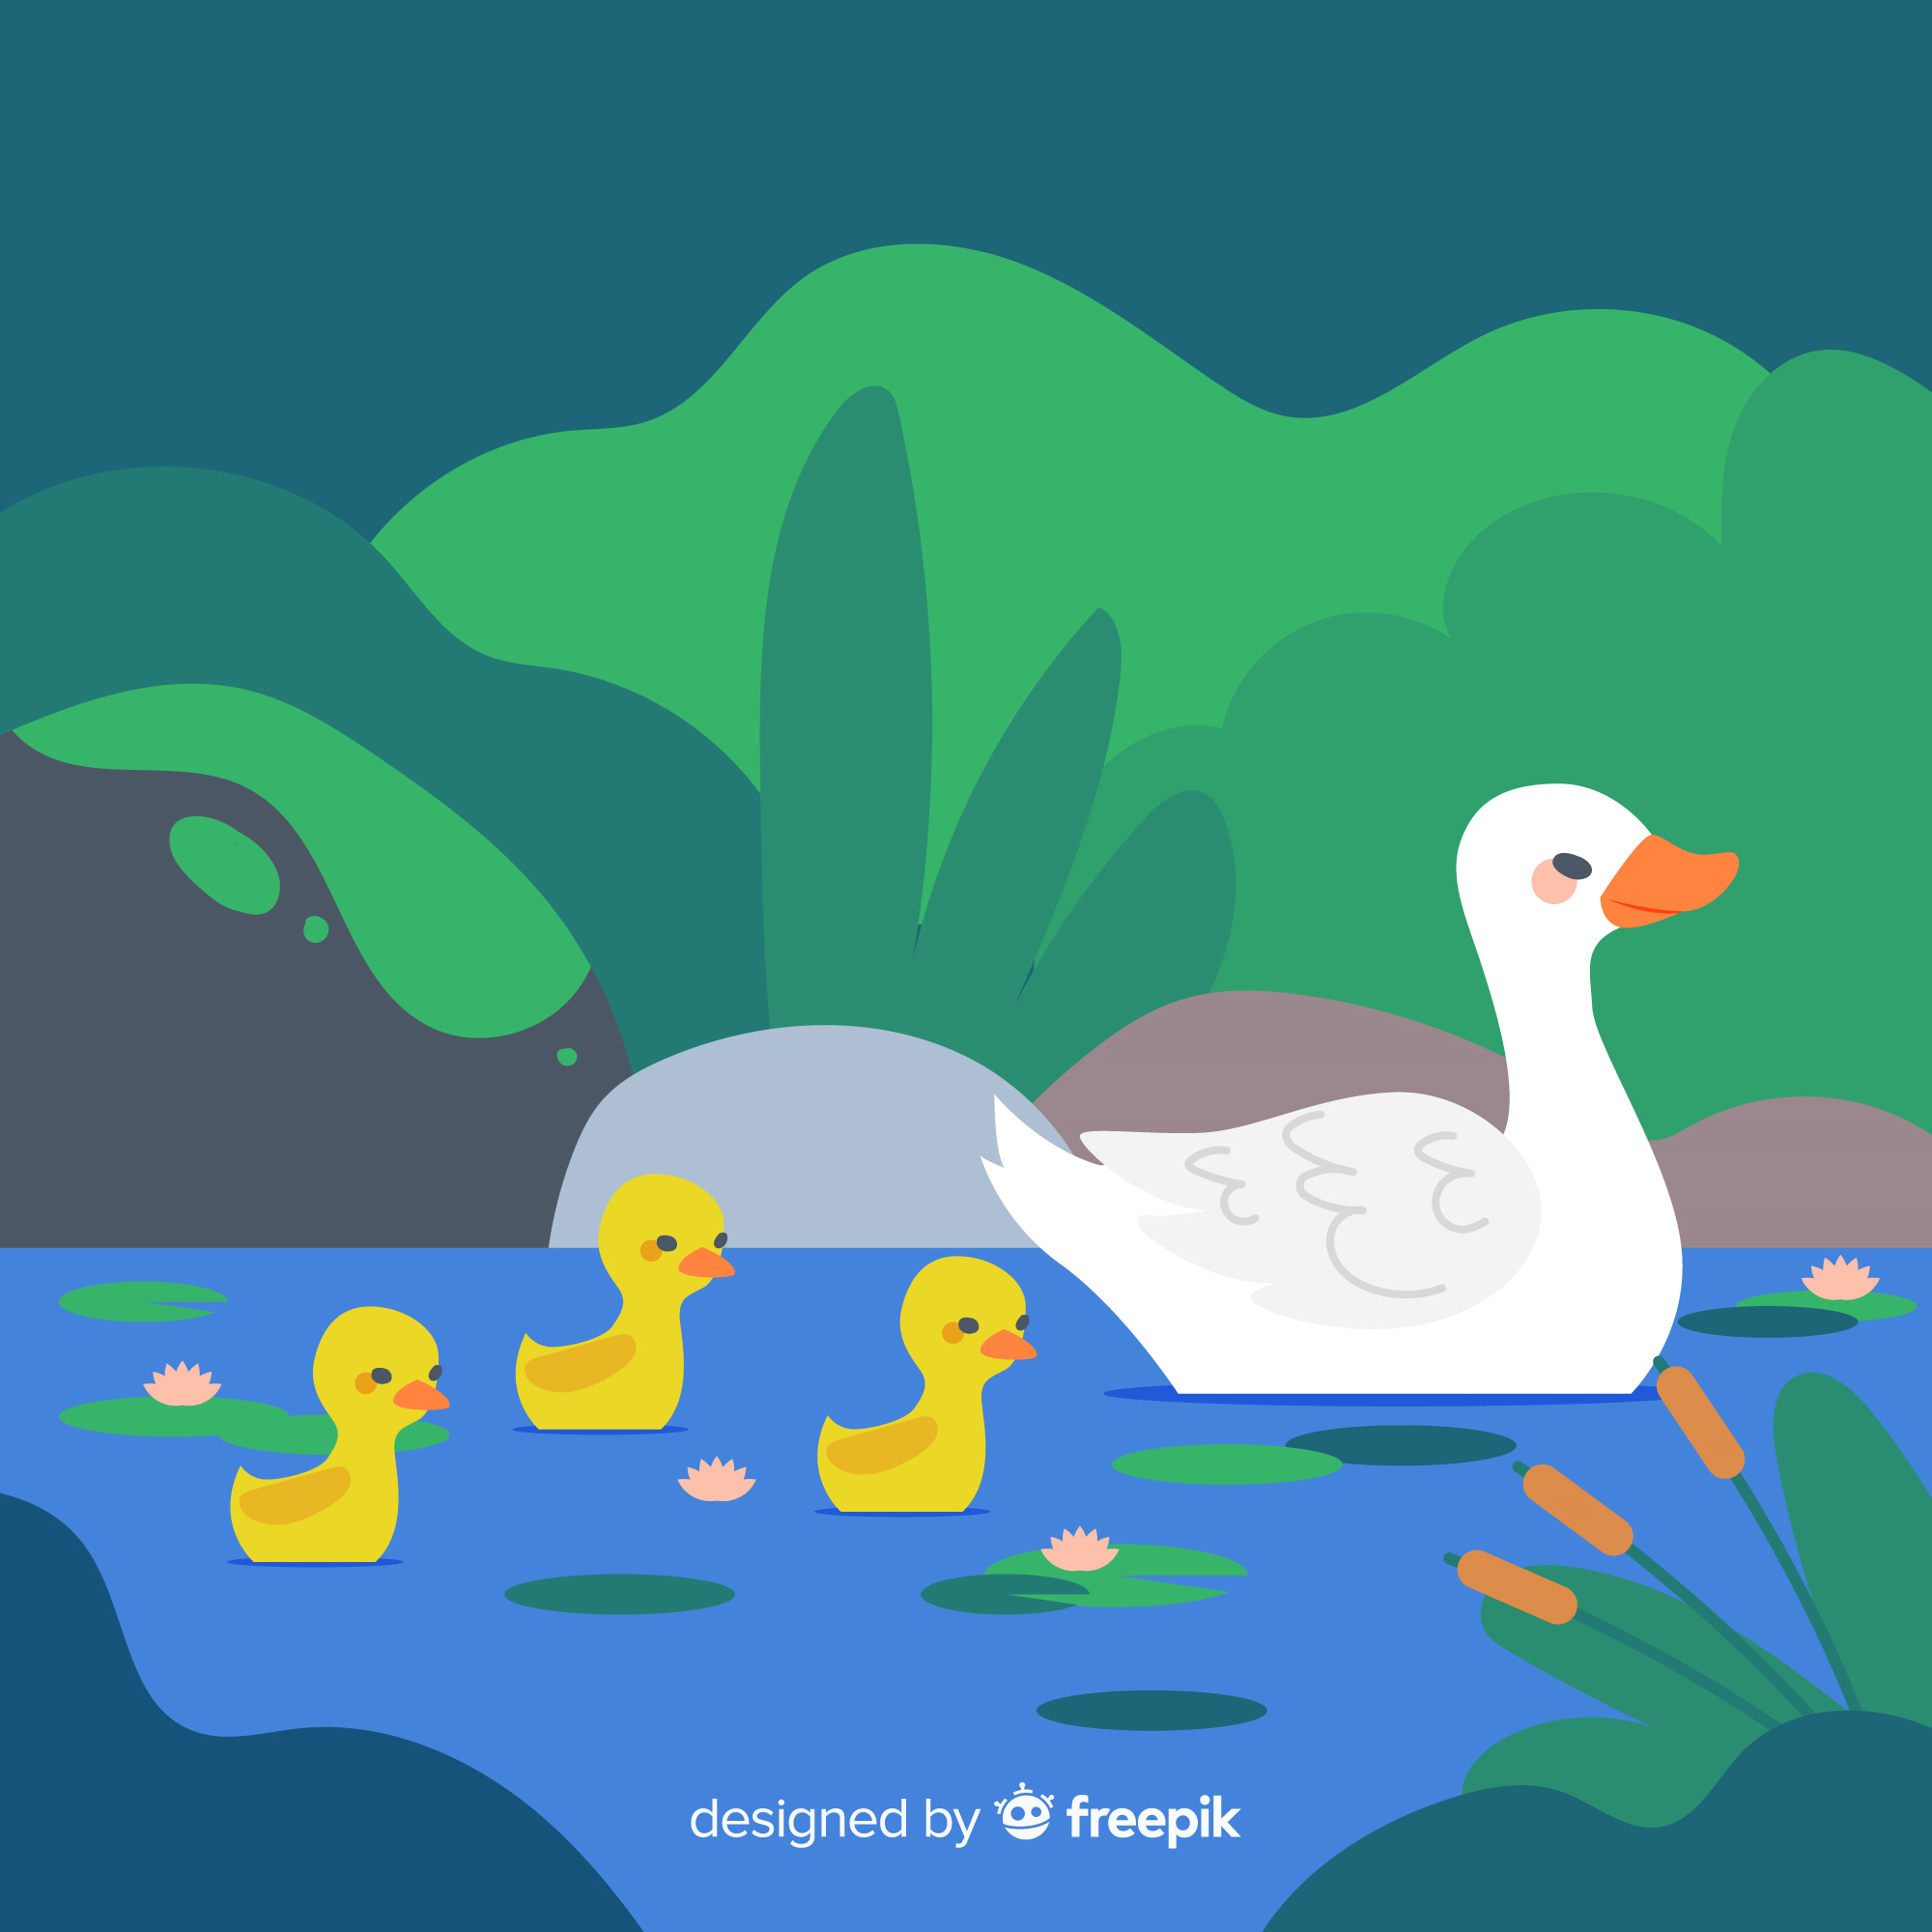
\includegraphics[width=.4\textwidth]{media/image252.png}

\item 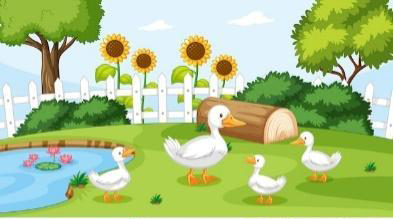
\includegraphics[width=.4\textwidth]{media/image253.png}
\end{escolha}
\end{multicols}

\pagebreak

\num{11} LEIA O TEXTO.

\begin{myquote}
\begin{verse}
\textbf{POMBINHA}

POMBINHA, QUANDO TU FORES,\\
ME ESCREVA PELO CAMINHO.\\
SE NÃO ACHARES PAPEL,\\
NAS ASAS DE UM PASSARINHO.

DO BICO FAZ UM TINTEIRO.\\
DA LÍNGUA PENA DOURADA.\\
DOS DENTES LETRA MIÚDA.\\
DOS OLHOS CARTA FECHADA.

A POMBINHA VOOU, VOOU\ldots{}\\
FOI-SE EMBORA E ME DEIXOU.
\end{verse}
\end{myquote}

O QUE ERA PARA FAZER COM OS OLHOS?

\begin{multicols}{2}
\begin{escolha}[itemsep=0pt]
\item TINTEIRO.

\item LETRA MIÚDA.

\item CARTA FECHADA.

\item PENA DOURADA.
\end{escolha}
\end{multicols}

\num{12} LEIA O TRECHO DE UMA HISTÓRIA.

\begin{myquote}
\textbf{CHAPEUZINHO VERMELHO}

ERA UMA VEZ UMA MENINA DE OLHOS NEGROS E LOUROS CABELOS CACHEADOS.

UM DIA, COM UM RETALHO DE TECIDO VERMELHO, SUA MÃE
COSTUROU PARA ELA UMA CURTA CAPA COM CAPUZ; FICOU UMA
BELEZINHA [\ldots{}].

\fonte{CONTOS TRADICIONAIS, FÁBULAS, LENDAS E MITOS. MINISTÉRIO DA EDUCAÇÃO. BRASÍLIA: FUNDESCOLA, 2000. P. 27.}
\end{myquote}

\pagebreak

ESSE TEXTO É DESTINADO A

%\begin{multicols}{2}
\begin{escolha}%[itemsep=-5pt]
\item JOVENS.

\item CRIANÇAS.

\item ADULTOS.

\item FAMÍLIAS.
\end{escolha}
%\end{multicols}

\num{13} A SEGUIR, APARECE O TRECHO INICIAL DE UMA HISTÓRIA. LEIA ESTE TEXTO COM ATENÇÃO.

\begin{myquote}
\textbf{NO REINO DAS LETRAS FELIZES}

EM UM REINO SOMENTE 
VIVIAM LETRAS, QUE JAMAIS SE UNIAM 
PARA FORMAR PALAVRAS. A RAINHA DECIDIU ACABAR COM ESSE 
SILÊNCIO. ELA CHAMOU SEUS CONSELHEIROS E DECRETOU:

--- ORGANIZEM UMA GRANDE FESTA E CONVIDEM TODAS AS 
LETRAS DO REINO. QUERO QUE AS LETRAS DO NOSSO REINO USEM 
A IMAGINAÇÃO E FAÇAM APRESENTAÇÕES PARA DEIXAR UMA MARCA 
ETERNA NA HISTÓRIA DO REINO.

\fonte{TEXTO ESCRITO PARA ESTE MATERIAL.}
\end{myquote}

DE QUE FALA O TEXTO?

\begin{escolha}
\item DA APRESENTAÇÃO DAS LETRAS.

\item DO SILÊNCIO DAS LETRAS.

\item DA TRISTEZA DAS LETRAS. 

\item DA ALEGRIA DAS LETRAS.
\end{escolha}

\pagebreak

\num{14} LEIA O TEXTO.

\begin{myquote}
\textbf{O GALO E A RAPOSA}

O GALO E AS GALINHAS VIRAM QUE LÁ LONGE VINHA UMA RAPOSA.

\begin{center}
\includegraphics[width=\textwidth]{media/image276.png}
\end{center}

EMPOLEIRARAM-SE NA ÁRVORE MAIS PRÓXIMA, PARA ESCAPAR DA INIMIGA.

COM SUA ESPERTEZA, A RAPOSA CHEGOU PERTO DA ÁRVORE E
SE DIRIGIU A ELES:

--- ORA, MEUS AMIGOS, PODEM DESCER DAÍ. NÃO SABEM QUE
FOI DECRETADA A PAZ ENTRE OS ANIMAIS? DESÇAM E VAMOS FESTEJAR ESSE
DIA TÃO FELIZ!

\fonte{DISPONÍVEL EM: \emph{http://www.dominiopublico.gov.br/download/texto/me001614.pdf}. ACESSO EM: 14 ABR. 2023.}
\end{myquote}

A RAPOSA QUERIA QUE O GALO E A GALINHA DESCESSEM DA ÁRVORE PARA

\begin{escolha}[itemsep=-5pt]
\item FAZER UMA FESTA.

\item COMÊ-LOS.

\item BRINCAR COM ELES.

\item CONTAR UM SEGREDO.
\end{escolha}

\pagebreak

\num{15} LEIA O DIÁLOGO. %E OBSERVE A IMAGEM.

%Paulo: Inserir imagem disponível no link: https://br.freepik.com/fotos-gratis/retrato-de-duas-irmas-afro-americanas-sorridentes_6873868.htm#page=2&query=boy%20giving%20girl%20a%20gift&position=8&from_view=search&track=ais.

%Disponível em: https://br.freepik.com/fotos-gratis/retrato-de-duas-irmas-afro-americanas-sorridentes_6873868.htm#page=2&query=boy%20giving%20girl%20a%20gift&position=8&from_view=search&track=ais. Acesso em: 19 abr. 2023.

\begin{myquote}
UMA MÃE DISSE:

--- TENHO UMA SURPRESA PARA VOCÊ, JULIANA.

--- O QUE É, MAMÃE?
\end{myquote}

\begin{figure}[H]
\centering
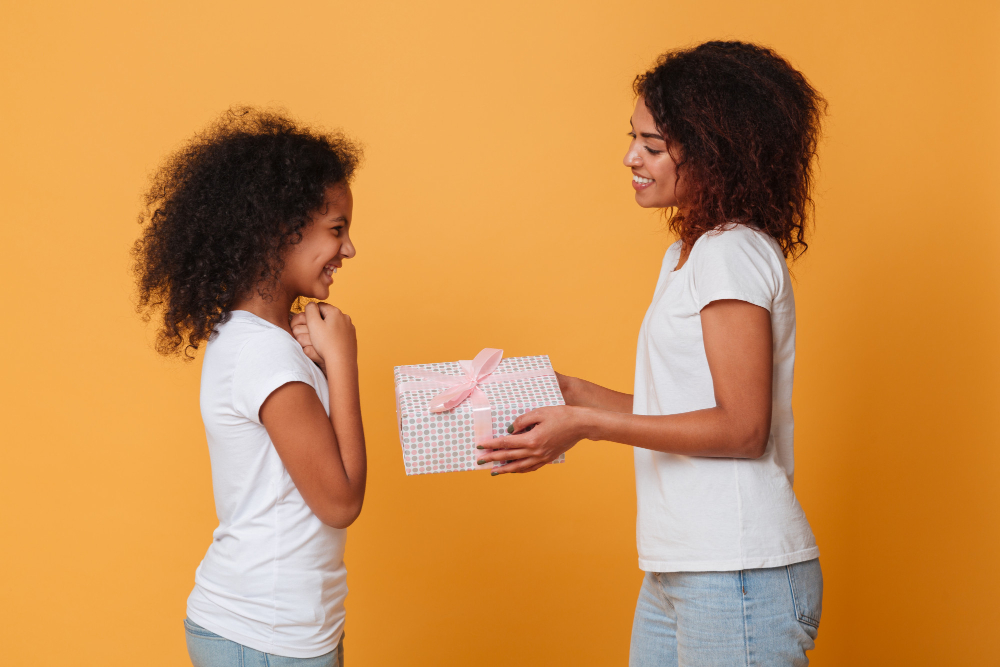
\includegraphics[width=.8\textwidth]{media/image259.png}
\end{figure}

\begin{myquote}
A MÃE RESPONDEU:

--- UM PRESENTE!

--- OH! MUITO OBRIGADA!
\end{myquote}

JULIANA, A FILHA, ESTÁ FELIZ PORQUE

\begin{escolha}
\item FOI VIAJAR.

\item GANHOU UM PRESENTE DE SUA MÃE.

\item ESTÁ BRINCANDO COM SEU GATINHO.

\item ESTÁ JOGANDO BOLA.
\end{escolha}


